\documentclass[aspectratio=43, dvipsnames]{beamer}
\usepackage[version=4]{mhchem}
\usepackage[aboveskip=1pt, belowskip=1pt]{caption}
\usepackage{amsmath}
\usepackage{siunitx}
\usepackage{pgfplots}
\pgfplotsset{compat=1.18,}
\usepgfplotslibrary{fillbetween}
\usepackage{tcolorbox}

% Command to display isotopes
\newcommand{\iso}[2]{\ce{^{#1}#2}}
% Command to write overlap
\newcommand{\overlap}[2]{\left\langle#1\middle\vert#2\right\rangle}
% Command to write Rs
\newcommand{\rs}{$\text{R}_{\text{S}}$ }
% Command to draw enumitems outside the environment
\newcommand{\enumitem}[1]{%
\setcounter{enumi}{#1}\usebeamertemplate{enumerate item}% 
}
% Set caption package options
\captionsetup{labelformat=empty}

\title[SF quenching]{Quenching of spectroscopic factors in \\ \texorpdfstring{\iso{10,12}{Be}(d, \iso{3}{He})}{10,12Be(d,3He)} reactions}
\date[October 2024]{Status by October 2024}
\author[M. Lozano et al.]{M. Lozano-González, A. Matta, B. Fernández-Domínguez,\texorpdfstring{\newline}{} F. Delaunay, J. Lois-Fuentes}
\institute{USC-IGFAE and LPC-Caen}

\usetheme{igfae}

\begin{document}

\maketitle

\section{Motivation}
\begin{frame}{A recap on spectroscopic factors}
    \textbf{Spectroscopic factors} shed light on the occupancy of single-particle states:
    \begin{equation*}
        \left.\frac{d\sigma}{d\Omega}\right\vert_{exp} = C^{2}S \cdot \left.\frac{d\sigma}{d\Omega}\right\vert_{s.p}, \quad \sum C^{2}S = (2j + 1) \text{ in IPSM}
    \end{equation*}
    % \begin{equation*}
    %     \left.\frac{d\sigma}{d\Omega}\right\vert_{exp} = C^{2}S \cdot \left.\frac{d\sigma}{d\Omega}\right\vert_{s.p}, \quad C^{2}S =\begin{cases}
    %         (2j + 1)\; \text{removing}     \\
    %         1\qquad\quad\,\, \text{adding} \\
    %     \end{cases} \text{ in IPSM}
    % \end{equation*}
    \begin{columns}[T]
        \begin{column}{0.48\linewidth}
            \hfill{}
            \begin{beamercolorbox}[sep=0.75em, center, wd=0.85\linewidth,rounded=true]{box1}
                \textbf{Experimentally:} Reduction of \sim\qty{65}{\percent}!
            \end{beamercolorbox}%
            \hfill{}
            \begin{itemize}
                \item \textbf{Short-range} correlations: tensor forces,...
                \item \textbf{Long-range}: vibrations, giant resonances,...
            \end{itemize}
        \end{column}
        \begin{column}{0.48\linewidth}
            \vspace{-1em}
            \begin{figure}
                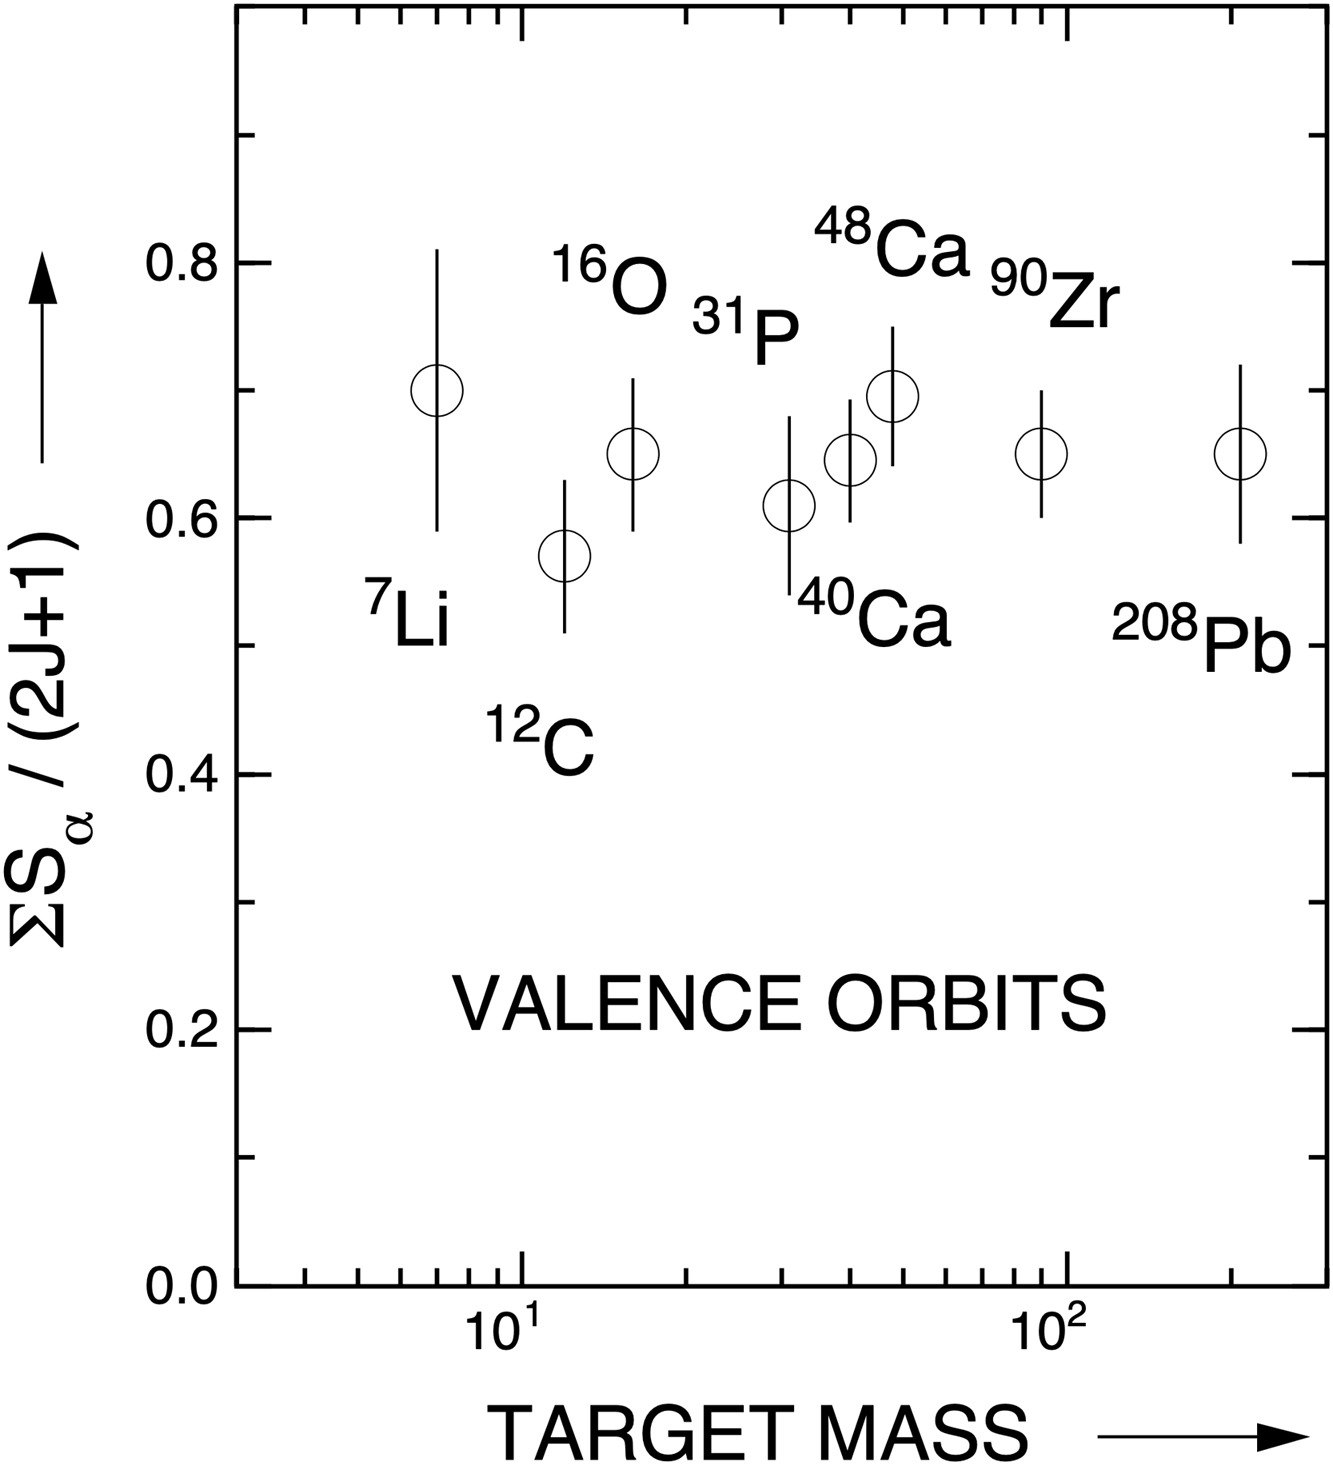
\includegraphics[width=0.725\linewidth]{figures/lapikas_review.jpg}
                \caption{L. Lapikás, Nuclear Phys. A 553 (1993)}
            \end{figure}
        \end{column}
    \end{columns}
\end{frame}

\begin{frame}{A long-standing puzzle}
    A trend with asymmetry energy $\Delta S \equiv S_{n} - S_{p}$ is found depending on the experimental \textbf{probe}!
    \begin{figure}
        \begin{tikzpicture}
            \node[anchor=south west,inner sep=0] (image) at (0,0) { 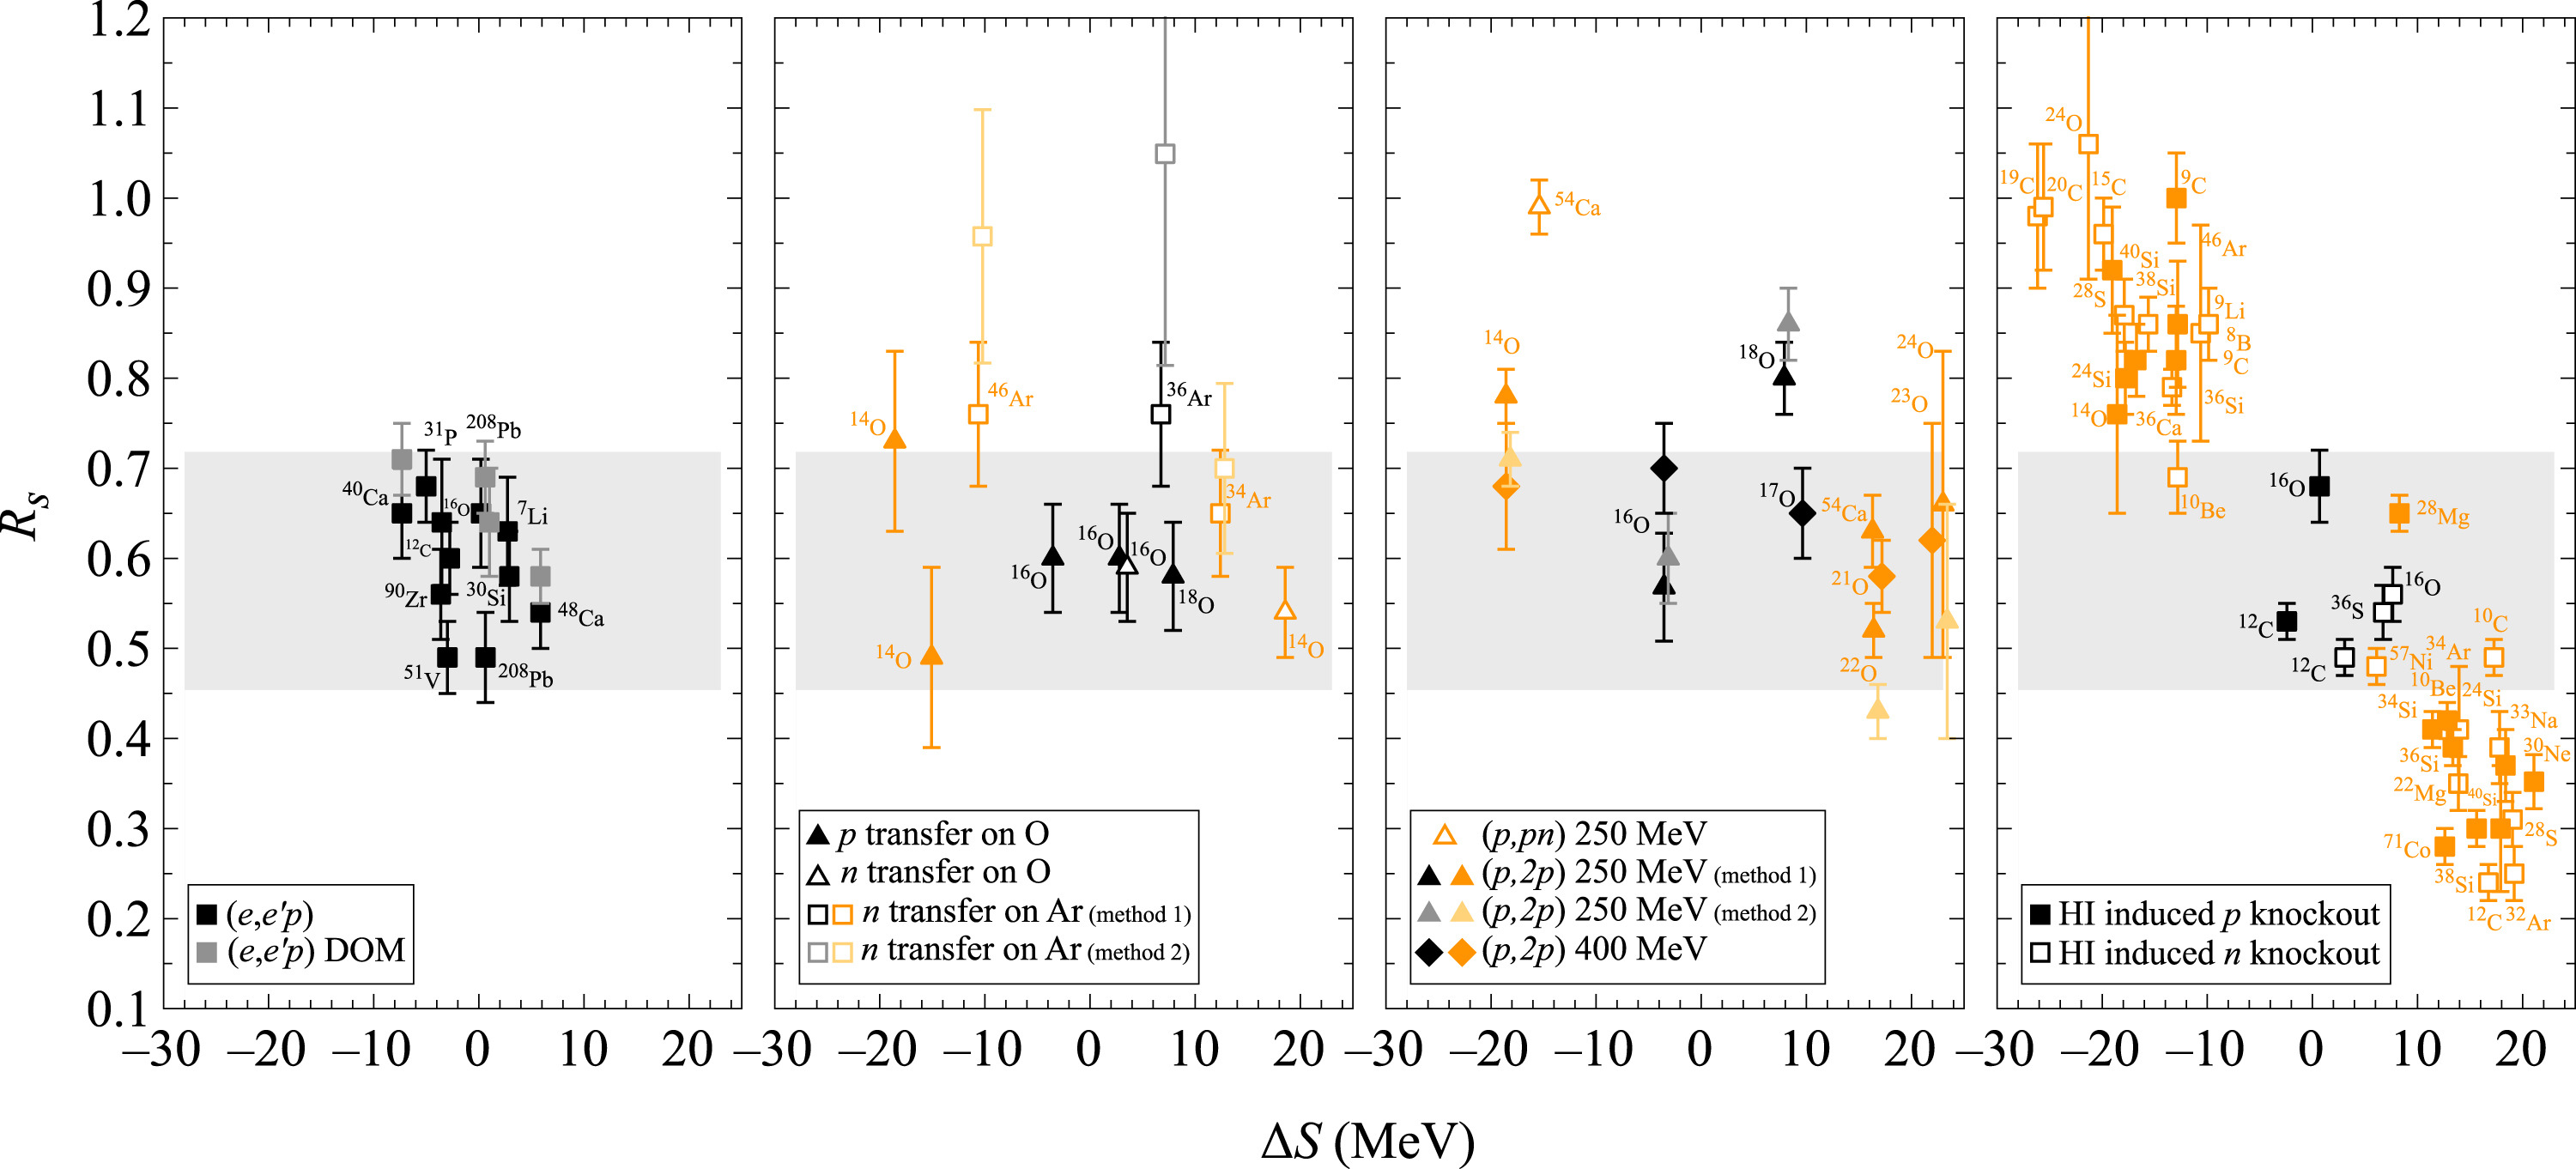
\includegraphics[width=0.9\linewidth]{figures/auman.jpg}
            };
            \myscope[false]{
                \node at (0.17, 0.9) {(e,e'p)};
                \node at (0.405, 0.9) {transfer};
                \node at (0.65, 0.9) {(p,2p)};
                \node[align=center] at (0.89, 0.9) {\textcolor{red}{Be-C} \\ \textcolor{red}{knock-out}};
                \draw[thick, red] (0.825, 0.78) -- (0.97, 0.335);
            }
        \end{tikzpicture}
        \caption{T. Aumann \textit{et al.} Prog. Part. Nucl. Phys. 118 (2021)}
    \end{figure}
    \mycolorbox{box2}{
        $\Rightarrow$ measure towards more exotic nuclei: $\left|\Delta S \right| \uparrow$
    }
\end{frame}

\begin{frame}[t]{Importance of GMF}
    Towards exotic nuclei (loosely bound or halo), a \textbf{\textit{geometrical mismatch factor}} emerges from the very different w.f. in the overlap:
    \vspace{-1em}
    \begin{columns}[T]
        \column{0.48\linewidth}
        {
            \begin{figure}
                \begin{tikzpicture}
                    \node[anchor=south west, inner sep=0pt] (image) at (0,0){
                        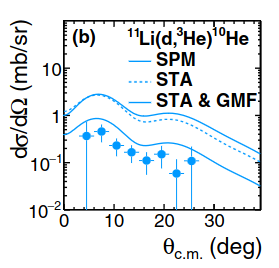
\includegraphics[width=0.7\linewidth]{figures/matta_11Li_d3He.png}};
                    \myscope[false]{
                        \draw[<-, very thick, magenta] (0.6, 0.46) -- (0.68, 0.54);
                        \draw[<-, very thick, magenta] (0.3, 0.55) -- (0.35, 0.65);
                    }
                \end{tikzpicture}
                \caption{A.Matta et al., Phys. Rev. C 92 (2015)}
            \end{figure}
        }
        \column{0.48\linewidth}
        {
            \begin{figure}
                \begin{tikzpicture}
                    \node[anchor=south west, inner sep=0pt] (image) at (0, 0){
                        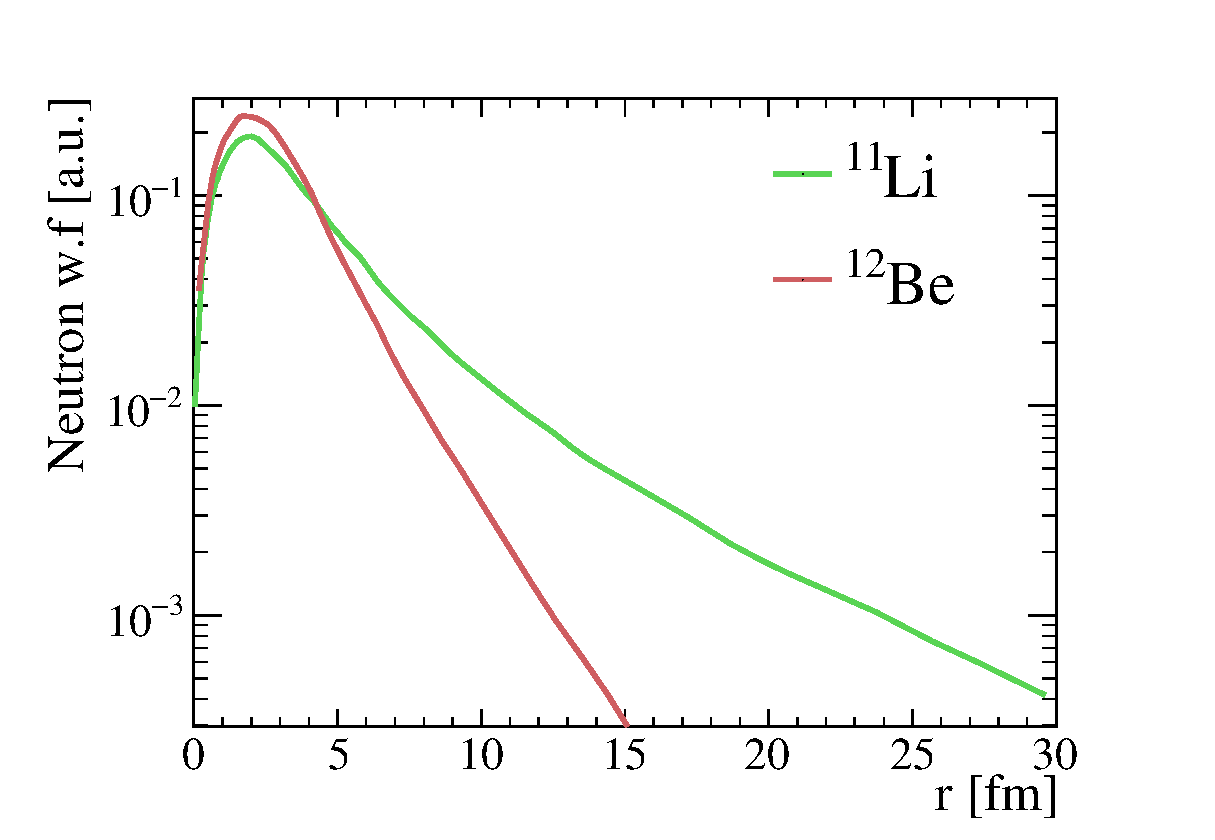
\includegraphics[width=1\linewidth]{figures/wfs.eps}};
                    \myscope[false]{
                        \draw[<->, very thick, dashed, magenta] (0.47, 0.25) -- (0.7, 0.25);
                    }
                \end{tikzpicture}
                \caption{N. K. Timofeyuk, private communication (in E748 proposal)}
            \end{figure}
        }
    \end{columns}
    \begin{columns}[c]
        \begin{column}{0.78\linewidth}
            \mycolorbox[1]{box4}{
                $\Rightarrow$ Need to correct $C^{2}S$ by its value!
            }
        \end{column}
    \end{columns}
    % \begin{column}{0.5\linewidth}
    %     \mycolorbox[0.95]{box4}{
    %         \begin{itemize}
    %             \item Measure $\left\langle\iso{10,12}{Be}\middle|\iso{9,11}{Li}\right\rangle$
    %             \item $\Delta S = -12.8 | -19.8 \unit{\MeV}$
    %         \end{itemize}
    %     }
    % \end{column}%
    % \begin{column}{0.5\linewidth}
    %     \mycolorbox{box1}{
    %         \begin{itemize}
    %             \item Establish systematics for \textbf{\color{magenta} GMF}
    %         \end{itemize}
    %     }
    % \end{column}
    % \end{columns}
\end{frame}

\begin{frame}{Physics case of E748}
    E748 @ GANIL back in 2017. Using \iso{10,12}{Be}(d,\iso{3}{He}) reactions to:
    \bigskip
    \begin{columns}[T]
        \begin{column}{0.52\linewidth}
            \mycolorbox[1]{box2}{
            $\text{R}_{\text{S}}$ and $\Delta S$ dependence:
            {\small
            \begin{itemize}
                \item $\left\langle\iso{10}{Be}\middle|\iso{9}{Li}\right\rangle, \Delta S = \qty{-12.8}{\MeV}$
                \item $\left\langle\iso{12}{Be}\middle|\iso{11}{Li}\right\rangle, \Delta S = \textcolor{magenta}{\qty{-19.8}{\MeV}}$
            \end{itemize}}
            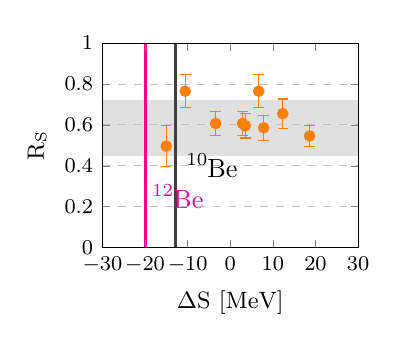
\begin{tikzpicture}[scale=0.95, trim left=-27]
                \begin{axis}[
                    footnotesize,
                    % width=0.5\linewidth,
                    % scale only axis,
                    xlabel={$\Delta$S [MeV]},
                    ylabel={$\text{R}_{\text{S}}$},
                    xmin=-30, xmax=30,
                    ymin=0, ymax=1,
                    ymajorgrids=true, yminorgrids=true,
                    grid style = {dashed},
                    axis on top,
                    ]
                    \addplot[fill=black!12, draw=none, forget plot] coordinates {(\pgfkeysvalueof{/pgfplots/xmin}, 0.45) (\pgfkeysvalueof{/pgfplots/xmax}, 0.45)  (\pgfkeysvalueof{/pgfplots/xmax}, 0.72) (\pgfkeysvalueof{/pgfplots/xmin}, 0.72)};
                    \addplot [orange, only marks,
                        error bars/.cd,
                        y dir=both, y explicit,
                    ] table [row sep=crcr, y error=u] {
                            x		   y      u
                            -18.508    0.732  0.103\\
                            -15.028    0.496  0.099\\
                            -10.552    0.765  0.080\\
                            -3.425    0.607  0.058\\
                            2.873    0.607  0.059\\
                            3.536    0.596  0.060\\
                            6.685    0.765  0.081\\
                            7.845    0.586  0.060\\
                            12.320    0.655  0.072\\
                            18.619    0.546  0.051\\
                        };
                    \draw[black!75, very thick] (axis cs:-12.8,\pgfkeysvalueof{/pgfplots/ymin}) -- (axis cs:-12.8,\pgfkeysvalueof{/pgfplots/ymax});
                    \node[right] at (-12.8, 0.4) {\iso{10}{Be}};
                    \draw[magenta, very thick] (axis cs:-19.8,\pgfkeysvalueof{/pgfplots/ymin}) -- (axis cs:-19.8,\pgfkeysvalueof{/pgfplots/ymax});
                    \node[magenta, right] at (-20.8, 0.25) {\iso{12}{Be}};
                \end{axis}
            \end{tikzpicture}
            }
        \end{column}
        \begin{column}{0.48\linewidth}
            \mycolorbox[1]{box3}{\small
                Explore effects of GMF:
                \begin{itemize}
                    \item $\left\langle\iso{10}{Be}\middle|\iso{9}{Li}\right\rangle, \text{GMF} \sim \num{1}$
                    \item $\left\langle\iso{12}{Be}\middle|\iso{11}{Li}\right\rangle, \text{GMF} \sim \textcolor{blue}{\num{0.5}?}$
                \end{itemize}
                \begin{tikzpicture}[
                        trim left=-27,
                    ]
                    \centering
                    \begin{axis}[
                        width=0.63\linewidth,
                        scale only axis,
                        ylabel={$\text{S}_{\text{2n}}$ [MeV]},
                        xticklabels={\iso{10}{Be}, \iso{9}{Li}, \iso{12}{Be}, \textcolor{magenta}{\iso{11}{Li}}},
                        xtick={1,2,3, 4},
                        xmin=0.75, xmax=4.25,
                        ymin=0, ymax=8.5,
                        ymajorgrids=true, yminorgrids=true,
                        % ytick distance=0.25,
                        grid style = {dashed},
                        % x tick label style = {font=\tiny},
                        ]
                        \addplot+ [
                            scatter/classes={
                                    a={blue},
                                    b={magenta}
                                },
                            scatter,
                            scatter src=explicit symbolic,
                        ] coordinates {
                                (1, 8.48) [a]
                                (2, 6.10) [a]
                                (3, 3.67) [a]
                                (4, 0.37) [b]
                            };
                    \end{axis}
                \end{tikzpicture}
            }
        \end{column}
    \end{columns}
\end{frame}

\section{Methodology}
\begin{frame}[c]{Experimental technique}
    Tradional solid target experiment @ LISE
    \vspace{1.5em}
    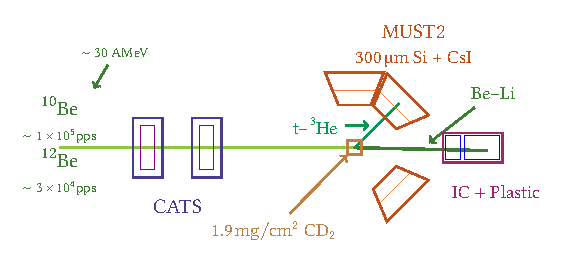
\includegraphics[width=1\linewidth]{figures/setup.pdf}
\end{frame}

\begin{frame}[t]{A glance at the analysis}
    \begin{columns}[T]
        \begin{column}{0.48\linewidth}
            \mycolorbox{box4}{
                \enumitem{1} \textbf{Heavy} ID at \qty{0}{\degree}
            }
            \begin{tikzpicture}
                \node[anchor = south west, inner sep = 0pt] (image) at (0,0){
                    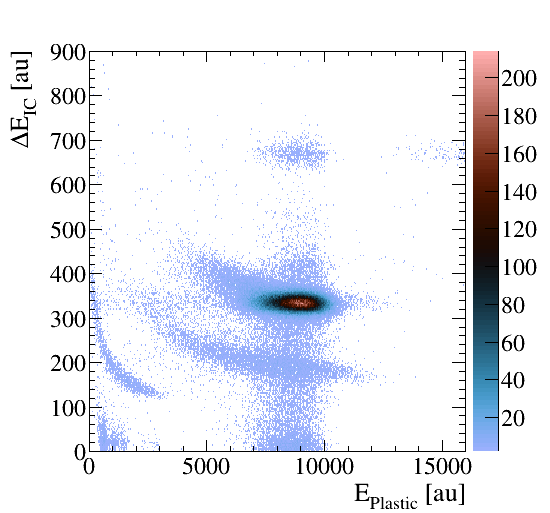
\includegraphics[width=1\linewidth]{figures/heavy.png}
                };
                \myscope[false]{
                \node[pin={
                [pin distance=5mm,
                        pin edge={<-, very thick, ForestGreen}]0:{Be}}
                ] at (0.60, 0.42) {};
                \node[pin={
                [pin distance=5mm,
                        pin edge={<-, very thick, color=ForestGreen}]0:{Li}}
                ] at (0.60, 0.28) {};
                }
            \end{tikzpicture}
        \end{column}
        \begin{column}{0.48\linewidth}
            \mycolorbox{box2}{
                \enumitem{2} \textbf{Light} PID in DSSD
            }
            \begin{tikzpicture}
                \node[anchor=south west, inner sep=0pt] (image) at(0,0){
                    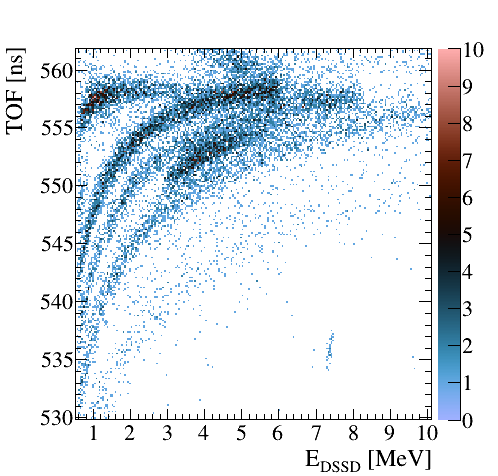
\includegraphics[width=1\linewidth]{figures/light.png}
                };
                \myscope[false]{
                    \node[pin={[pin distance=16mm, pin edge={<-, line width = 1.5pt, orange}]-87:A = 1}] at (0.2, 0.65) {};
                    \node[pin={[pin distance = 10mm, pin edge={<-, line width=1.5pt, orange}]-80:A = 2}] at (0.25, 0.65) {};
                    \node[pin={[pin distance=8mm, pin edge={<-, line width=1.5pt, orange}]-70:A = 3}] at (0.4, 0.7) {};
                    \node[pin={[pin distance=4mm, pin edge={<-, line width = 1.5pt, orange}]-75:A = 4}] at (0.6, 0.72) {};
                }
            \end{tikzpicture}
        \end{column}
    \end{columns}
    \mycolorbox{box1}{
        \enumitem{3} $E_{x}$ from \textbf{missing mass technique}
        $E_{\textrm{beam}} + (E,\theta)_{\textrm{Lab}} \rightarrow E_{x}$
    }
\end{frame}

\section{Results}
\begin{frame}[c]{Results: \texorpdfstring{\iso{10}{Be}(d,d)\iso{10}{Be} }{10Be(d,d)10Be}}
    \only<+>{
        Useful for normalization purpouses.
        \begin{columns}[c]
            \begin{column}{0.5\linewidth}
                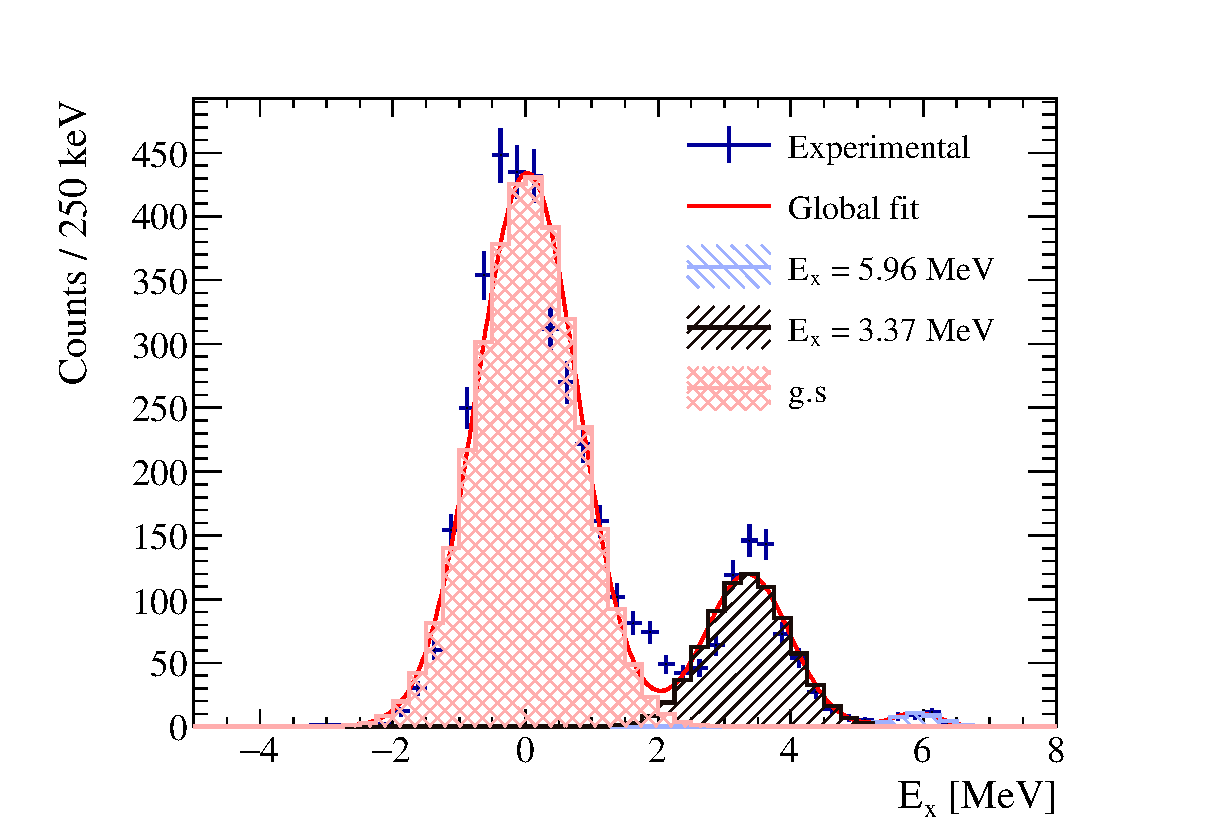
\includegraphics[width=\linewidth]{figures/10Be_dd_fit.eps}
            \end{column}\hfill
            \begin{column}{0.5\linewidth}
                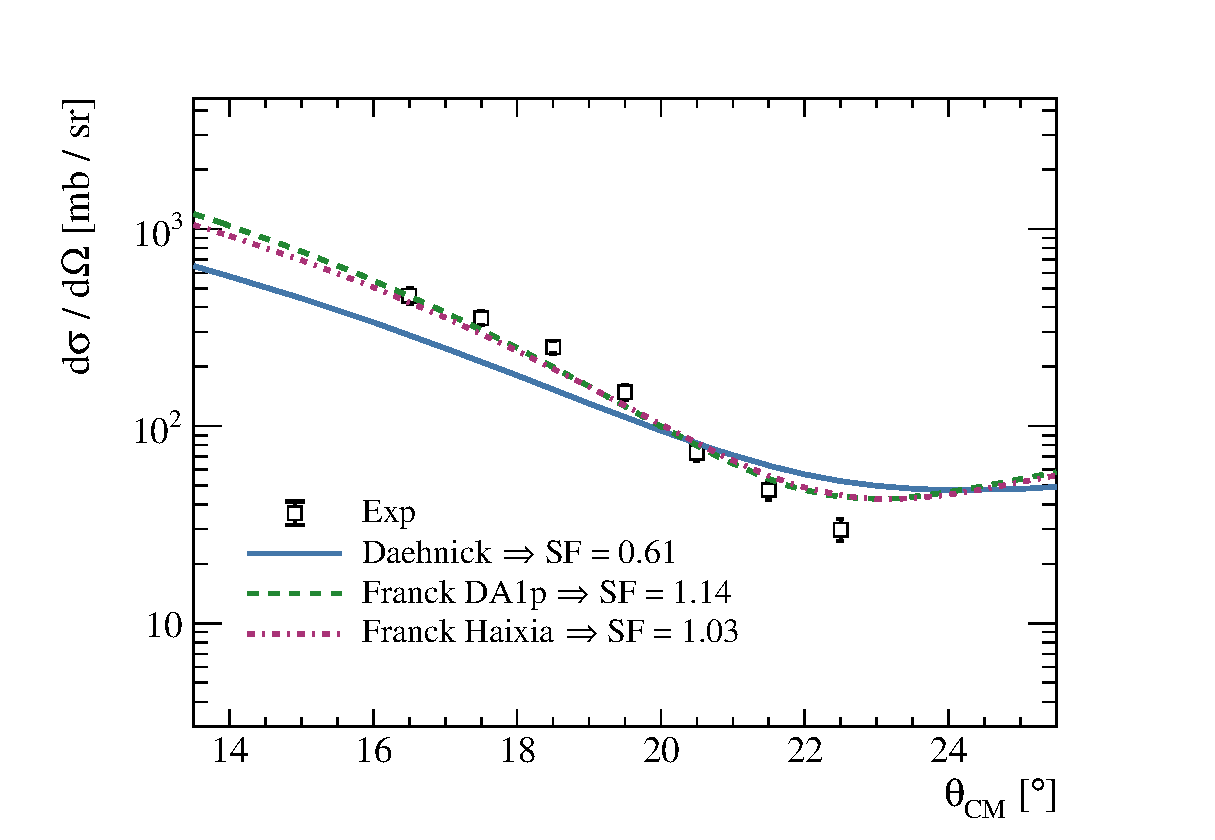
\includegraphics[width=\linewidth]{figures/10Be_dd_g0.eps}
            \end{column}
        \end{columns}
        \bigskip
        \mycolorbox{box2}{
            Best fit is provided by newer \textbf{Haixia} OMP.
        }
    }
    \only<+>{
        Experimental cross-section formula:
        \begin{equation*}
            \frac{d\sigma}{d\Omega} = \frac{N}{N_{\text{beam}} \textcolor{red}{N_{\text{targets}}} \textcolor{red}{\epsilon} \Delta \Omega}
        \end{equation*}
        \begin{columns}[c]
            \begin{column}{0.5\linewidth}
                \mycolorbox[0.95]{box2}{
                    \enumitem{1} \textbf{Target thickness} not measured during experiment:
                    \begin{itemize}
                        \item Set it from normalization of elastic
                        \item \textbf{Ongoing}: fix it from simulation
                    \end{itemize}}
            \end{column}\hfill
            \begin{column}{0.5\linewidth}
                \mycolorbox[0.95]{box4}{
                    \enumitem{2} ZDD had a poor performance. Averaged $\epsilon$:
                    \begin{itemize}
                        \item IC: \qty{30}{\percent}
                        \item Plastic: \qty{50}{\percent}
                    \end{itemize}}
            \end{column}
        \end{columns}
    }
\end{frame}

\begin{frame}[t]{Results: \texorpdfstring{\iso{10}{Be}(d,t)\iso{9}{Be} }{10Be(d,t)9Be}}
    Relatively high statistics. Used for benchmarking analysis routines.

    \begin{columns}[c]
        \begin{column}{0.5\linewidth}
            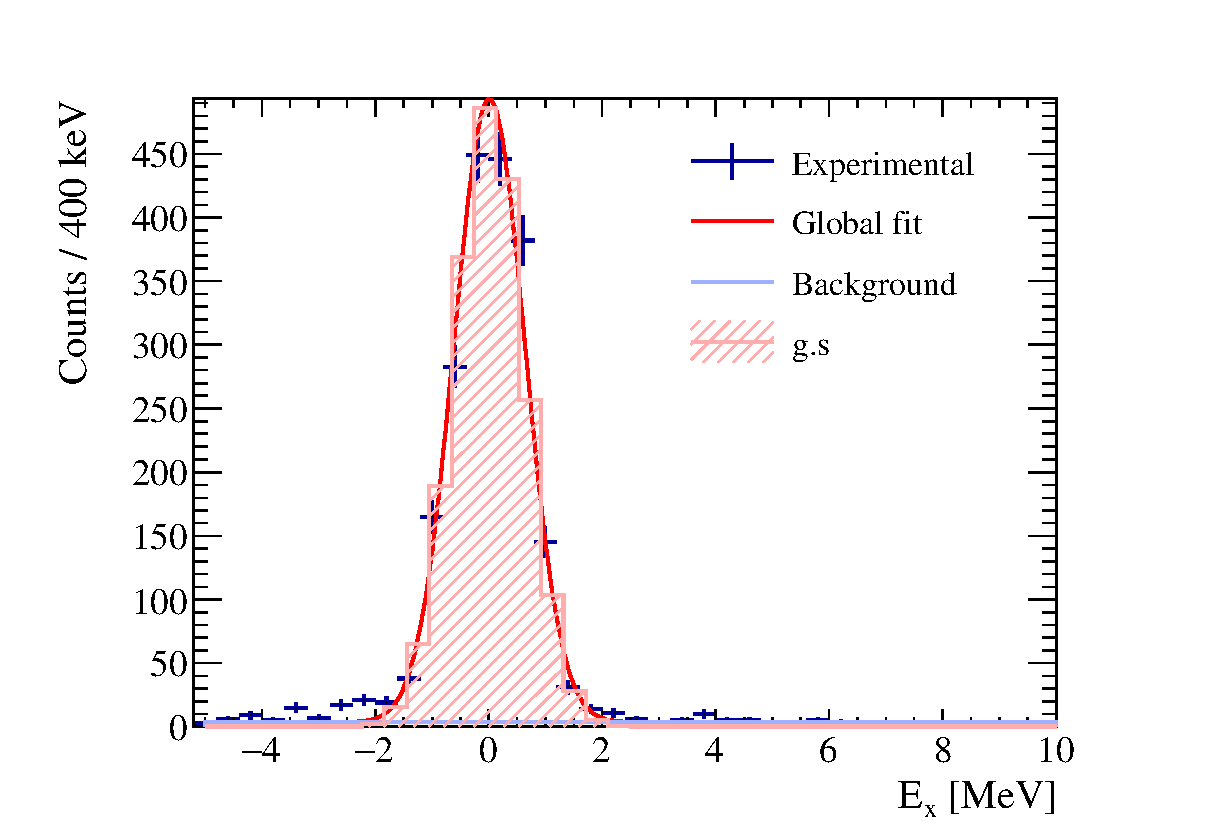
\includegraphics[width=\linewidth]{figures/10Be_dt_fit.eps}
        \end{column}\hfill
        \begin{column}{0.5\linewidth}
            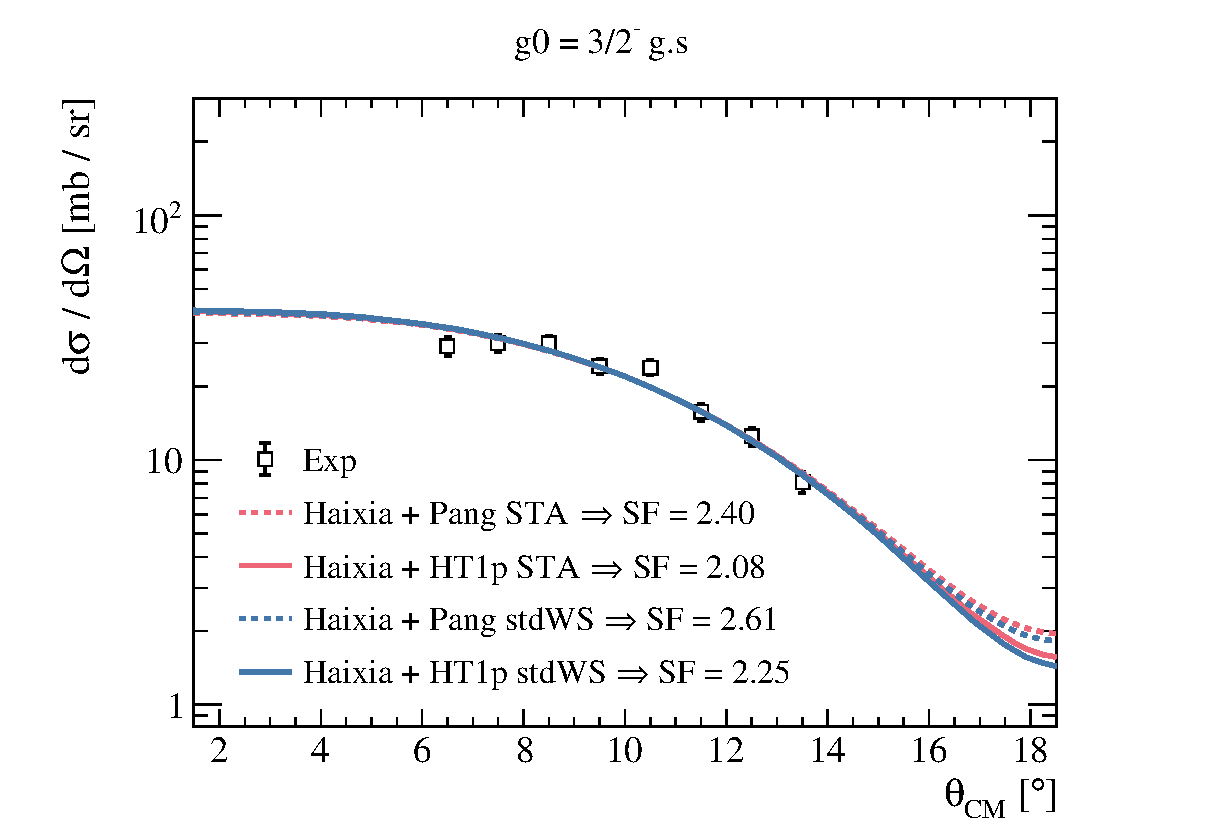
\includegraphics[width=\linewidth]{figures/10Be_dt_g0.eps}
        \end{column}
    \end{columns}

    \begin{columns}
        \begin{column}{0.5\linewidth}
            \mycolorbox{box3}{
            \textbf{STA} prediction:
            $C^2S = \qty{1.50}{}$\\
            Our result:
            $C^2S_{\text{exp}} = \qty{2.08}{}$
            }
        \end{column}\hfill
        \begin{column}{0.5\linewidth}
            \mycolorbox{box4}{
                SFO-tls shell-model:
                $C^2S = \qty{2.51}{}$
            }
        \end{column}
    \end{columns}
\end{frame}

\begin{frame}[t]{Results: \texorpdfstring{\iso{10}{Be}(d,\iso{3}{He})\iso{9}{Li} }{10Be(d,3He)9Li}}
    \only<+>{
        \begin{columns}
            \begin{column}{0.5\linewidth}
                $3/2^-$ ground state and $1/2^-$ 1st excited state.
                \includegraphics[width=\linewidth]{figures/10Be_d3He_fit.eps}
            \end{column}\hfill
            \begin{column}{0.5\linewidth}
                \vspace{-2.5em}
                \begin{tikzpicture}
                    \node[anchor=south] (image) at (0,0){
                        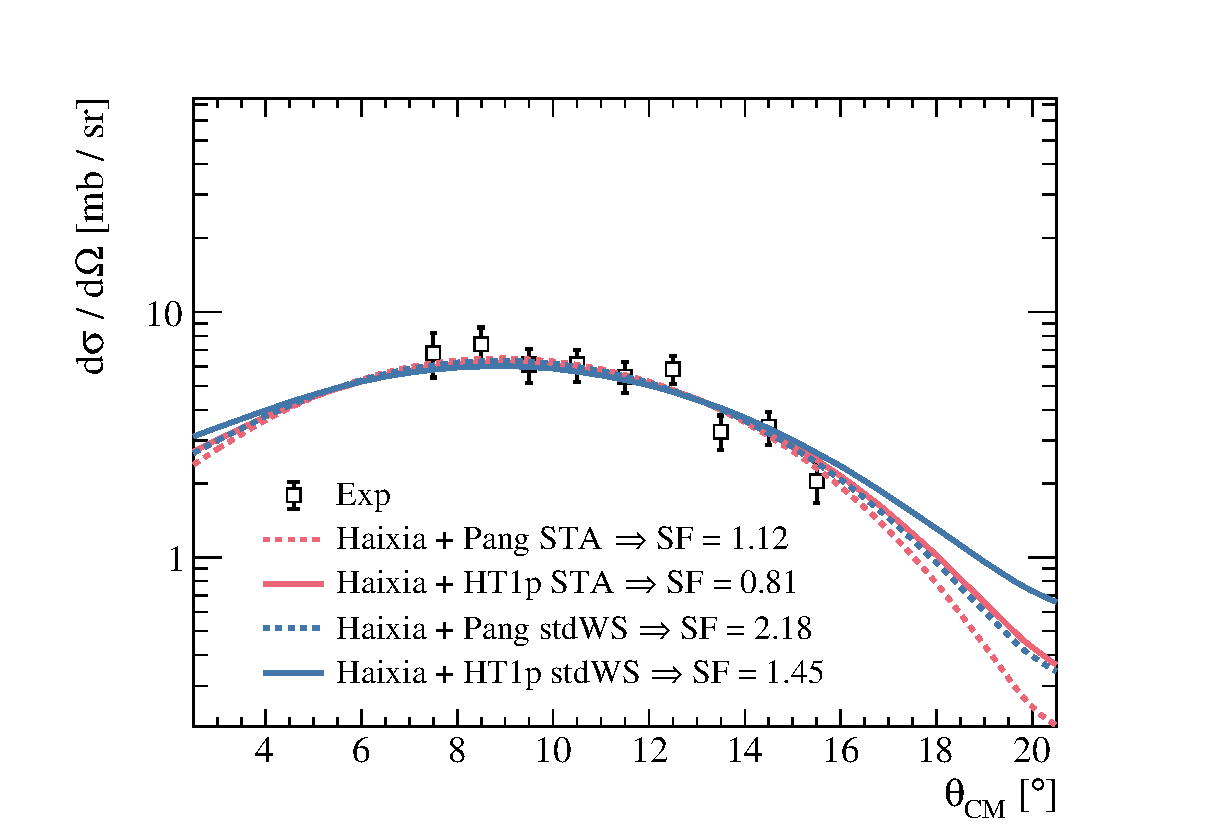
\includegraphics[width=\linewidth]{figures/10Be_d3He_g0.eps}
                    };
                    \node[align=center] (title) at (current bounding box.north) {Ground state};
                \end{tikzpicture}
                \begin{tikzpicture}
                    \node[anchor=south] (image) at (0,0){
                        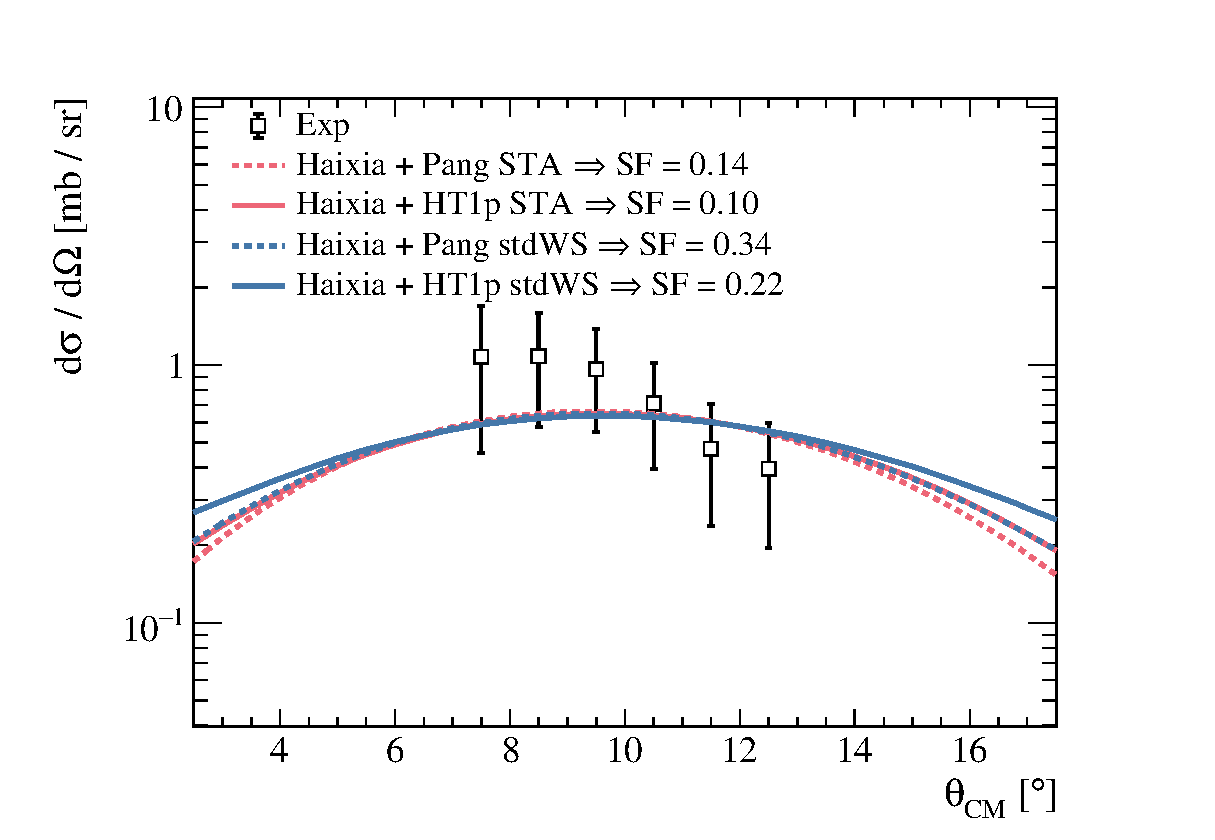
\includegraphics[width=\linewidth]{figures/10Be_d3He_g1.eps}
                    };
                    \node[align=center] (title) at (current bounding box.north) {1st excited};
                \end{tikzpicture}
            \end{column}
        \end{columns}
    }
    \only<+>{
        \begin{columns}[T]
            \begin{column}{0.5\linewidth}
                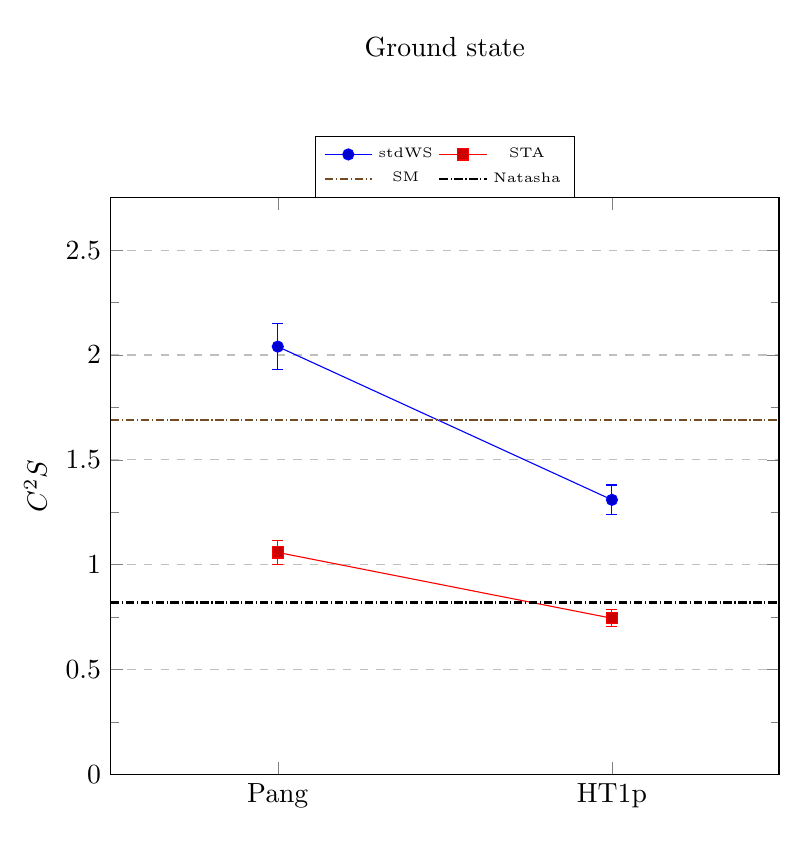
\begin{tikzpicture}[
                        % background rectangle/.style={fill=white},
                        % show background rectangle,
                        trim left=-30,
                    ]
                    \centering
                    \begin{axis}[
                            width=0.7\linewidth,
                            scale only axis,
                            title={Ground state},
                            title style={anchor=south, at={(0.5, 1.2)}},
                            % xlabel={Potential},
                            ylabel={$C^{2}S$},
                            minor y tick num=1,
                            xticklabels={Pang, HT1p},
                            xtick={1,2},
                            xmin=0.5, xmax=2.5,
                            ymin=0, ymax=2.75,
                            ymajorgrids=true, yminorgrids=false,
                            ytick distance=0.5,
                            legend style={
                                    fill=none,
                                    anchor=south,
                                    at={(0.5, 1.0)},
                                    font=\tiny,
                                },
                            legend columns=2,
                            grid style = {dashed},
                        ]
                        \addplot+ [
                            error bars/.cd,
                            y dir=both,y explicit,
                        ] coordinates {
                                (1, 2.04) +- (0,0.11)
                                (2, 1.309) +- (0,0.071)
                            };
                        \addplot+ [
                            error bars/.cd,
                            y dir=both,y explicit,
                        ] coordinates {
                                (1, 1.058) +- (0,0.058)
                                (2, 0.744) +- (0,0.040)
                            };
                        % \addplot+ [mark=none, densely dashdotted, thick] coordinates {(\pgfkeysvalueof{/pgfplots/xmin}, 1.159) (\pgfkeysvalueof{/pgfplots/xmax}, 1.159)};
                        \addplot+ [mark=none, densely dashdotted, thick] coordinates {(\pgfkeysvalueof{/pgfplots/xmin}, 1.690) (\pgfkeysvalueof{/pgfplots/xmax}, 1.690)};
                        \addplot+ [mark=none, densely dashdotted, thick] coordinates {(\pgfkeysvalueof{/pgfplots/xmin}, 0.819) (\pgfkeysvalueof{/pgfplots/xmax}, 0.819)};
                        \legend{stdWS, STA, SM, Natasha}
                    \end{axis}
                \end{tikzpicture}
                \par
                \mycolorbox{box4}{
                    \textbf{STA} fit agrees with N. Timofeyuk prediction!
                }
            \end{column}\hfill
            \begin{column}{0.5\linewidth}
                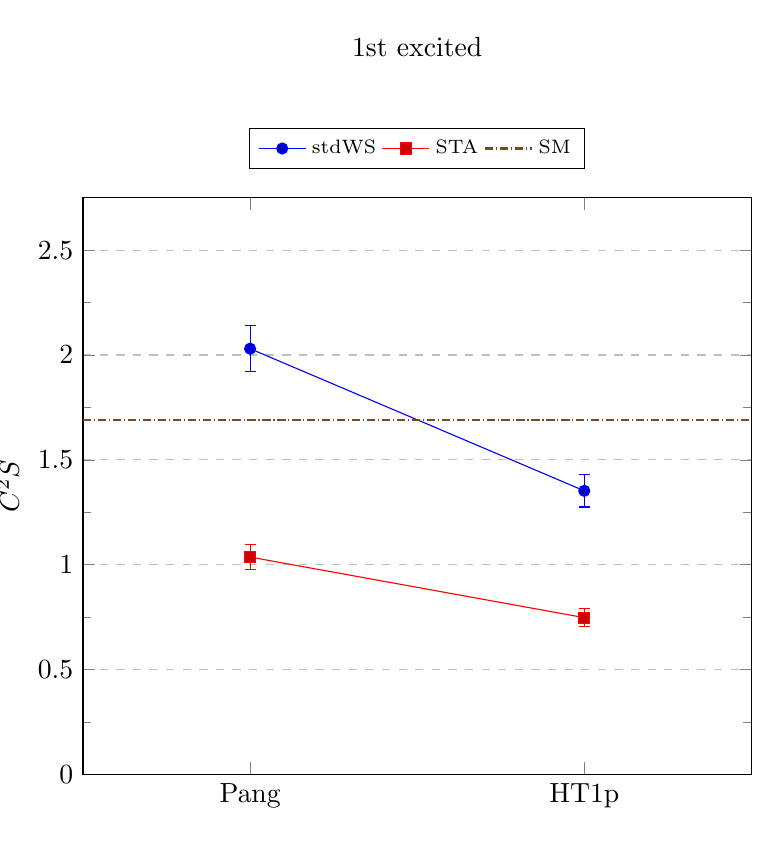
\begin{tikzpicture}[
                        % background rectangle/.style={fill=white},
                        % show background rectangle,
                        trim left=-20,
                    ]
                    \centering
                    \begin{axis}[
                            width=0.7\linewidth,
                            scale only axis,
                            title={1st excited},
                            title style={anchor=south, at={(0.5, 1.2)}},
                            % xlabel={Potential},
                            ylabel={$C^{2}S$},
                            minor y tick num=1,
                            xticklabels={Pang, HT1p},
                            xtick={1,2},
                            xmin=0.5, xmax=2.5,
                            ymin=0, ymax=2.75,
                            ymajorgrids=true, yminorgrids=false,
                            ytick distance=0.5,
                            legend style={
                                    fill=none,
                                    anchor=south,
                                    at={(0.5, 1.05)},
                                    font=\scriptsize,
                                },
                            legend columns=3,
                            grid style = {dashed},
                        ]
                        \addplot+ [
                            error bars/.cd,
                            y dir=both,y explicit,
                        ] coordinates {
                                (1, 2.03) +- (0,0.11)
                                (2, 1.352) +- (0,0.077)
                            };
                        \addplot+ [
                            error bars/.cd,
                            y dir=both,y explicit,
                        ] coordinates {
                                (1, 1.036) +- (0,0.058)
                                (2, 0.747) +- (0,0.042)
                            };
                        \addplot+ [mark=none, densely dashdotted, thick] coordinates {(\pgfkeysvalueof{/pgfplots/xmin}, 1.690) (\pgfkeysvalueof{/pgfplots/xmax}, 1.690)};
                        \legend{stdWS, STA, SM}
                    \end{axis}
                \end{tikzpicture}
                \par
                \mycolorbox{box2}{
                    \textbf{First} direct measurement!
                }
            \end{column}
        \end{columns}
    }
\end{frame}

\begin{frame}[t]{Results: \texorpdfstring{\iso{12}{Be}(d,d)\iso{12}{Be} }{12Be(d,d)12Be}}
    As before, this is used for setting the normalization of all channels.
    \begin{columns}[c]
        \begin{column}{0.5\linewidth}
            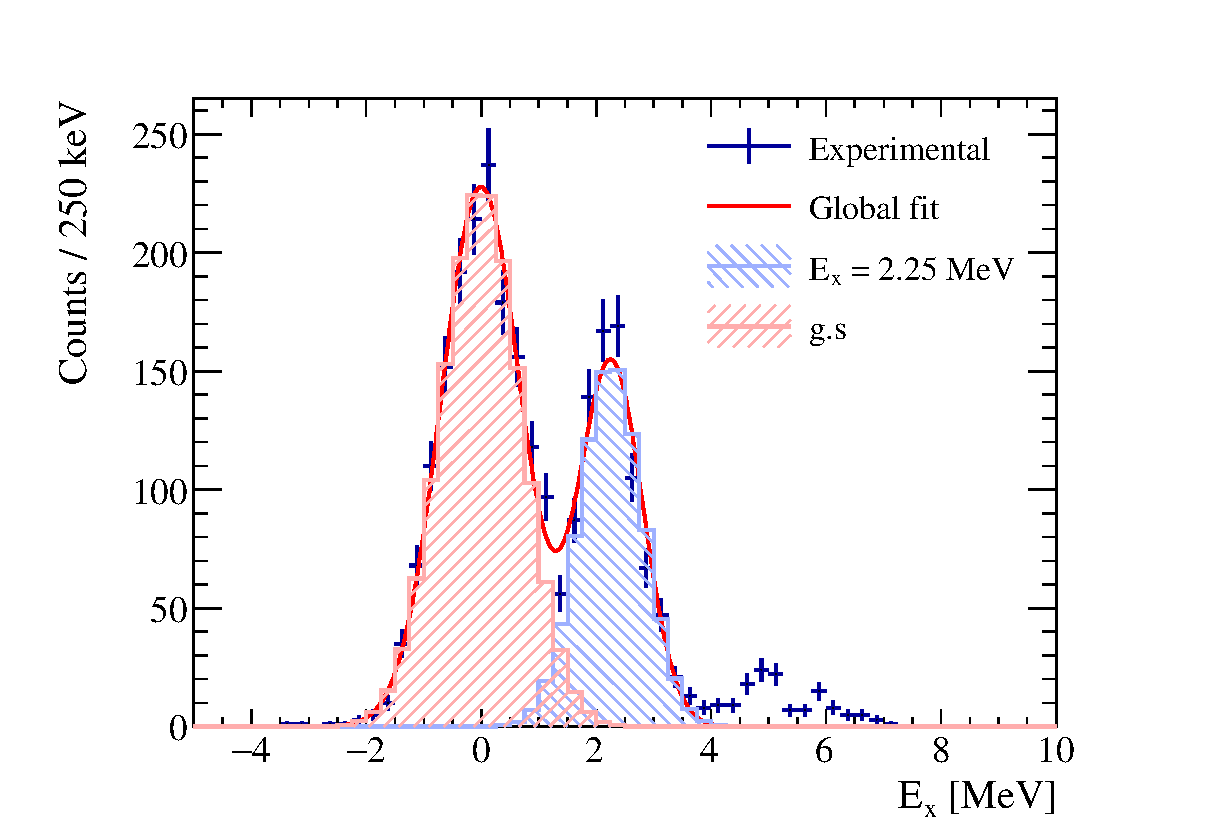
\includegraphics[width=\linewidth]{figures/12Be_dd_fit.eps}
        \end{column}\hfill
        \begin{column}{0.5\linewidth}
            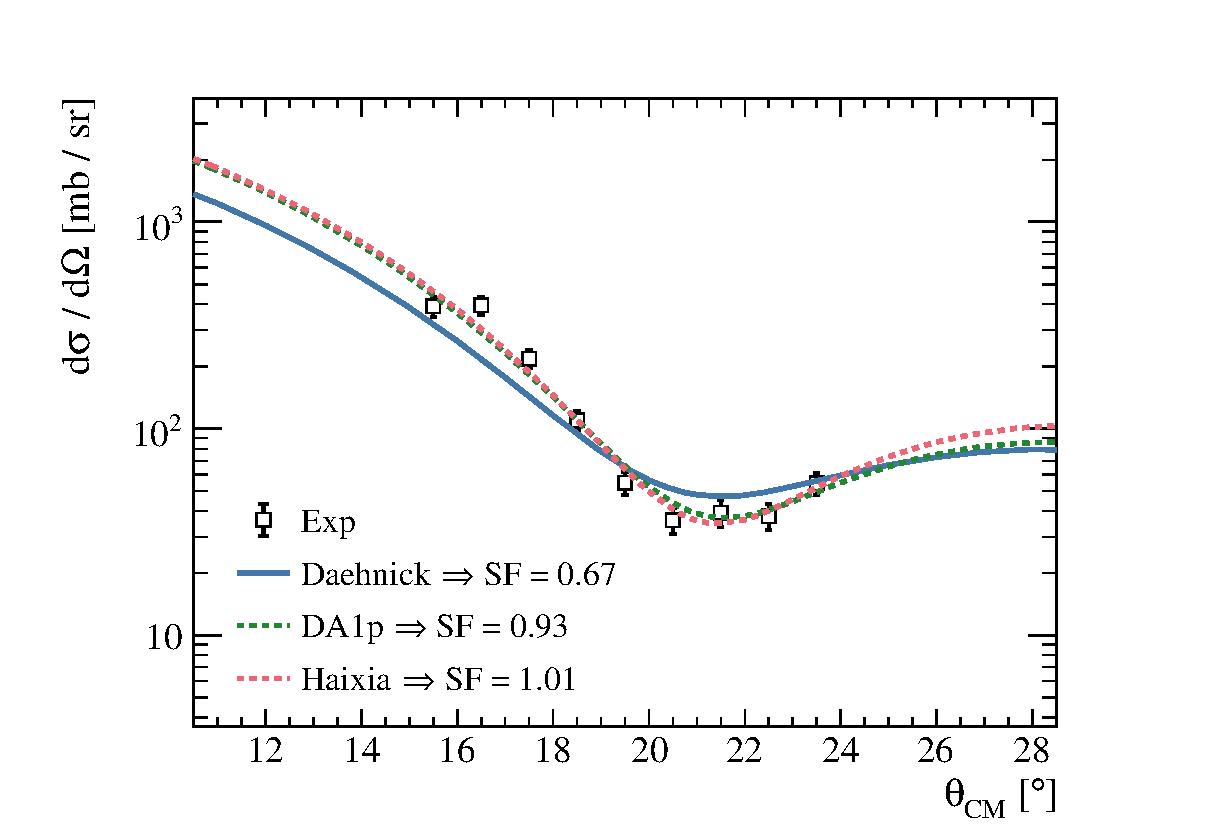
\includegraphics[width=\linewidth]{figures/12Be_dd_g0.eps}
        \end{column}
    \end{columns}
    \bigskip
    \mycolorbox{box2}{
        $N_{\text{targets}}$ is determined from the weighted average of this and the \iso{10}{Be}(d,d) result
    }
\end{frame}

\begin{frame}[t]{Results: \texorpdfstring{\iso{12}{Be}(d,\iso{3}{He})\iso{11}{Li} }{12Be(d,3He)11Li}}
    \only<1,2>{%
    So far only the \textbf{ground state} $3/2^{-}$ ($\ell = 1$) is analyzed.
    \begin{columns}[c]
        \begin{column}{0.5\linewidth}
            \only<1>{%
                \vspace{1.25em}
                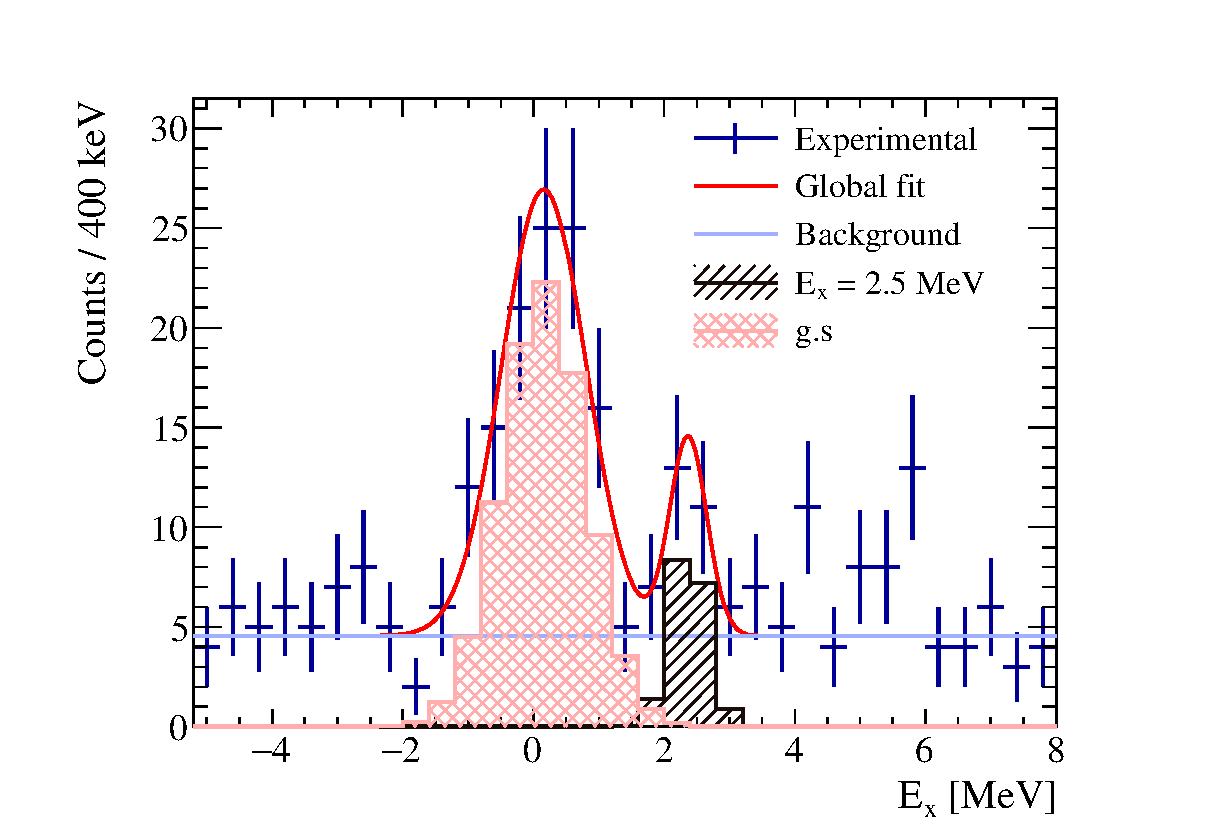
\includegraphics[width=\textwidth]{figures/12Be_d3He_fit.eps}
            }%
            \only<2>{%
                \begin{tikzpicture}[
                        trim left=-30,
                    ]
                    \centering
                    \begin{axis}[
                            width=0.7\linewidth,
                            scale only axis,
                            xlabel={Potential},
                            ylabel={$C^{2}S$},
                            minor y tick num=2,
                            xticklabels={Pang, HT1p},
                            xtick={1,2},
                            xmin=0.5, xmax=2.5,
                            ymin=0.1, ymax=2,
                            ymajorgrids=true, yminorgrids=false,
                            % ytick distance=0.25,
                            legend style={
                                    fill=none,
                                    anchor=south,
                                    at={(0.5, 1.05)},
                                    font=\scriptsize,
                                },
                            legend columns=3,
                            grid style={dashed, very thin},
                        ]
                        \addplot+ [
                            error bars/.cd,
                            y dir=both,y explicit,
                        ] coordinates {
                                (1, 0.647) +- (0,0.11)
                                (2, 0.310) +- (0,0.051)
                            };
                        \addplot+ [mark=none, densely dashdotted, thick] coordinates {(\pgfkeysvalueof{/pgfplots/xmin}, 1.642) (\pgfkeysvalueof{/pgfplots/xmax}, 1.642)};
                        \legend{stdWS, SM}
                    \end{axis}
                \end{tikzpicture}
            }
        \end{column}
        \begin{column}{0.5\linewidth}
            \includegraphics<1,2>[width=\textwidth]{figures/12Be_d3He_g0.eps}

        \end{column}
    \end{columns}
    \only<1>{
        \begin{columns}[c]
            \begin{column}{0.5\linewidth}
                \mycolorbox[1]{box2}{
                    Much lower cross section!
                }
            \end{column}
            \begin{column}{0.5\linewidth}
                \mycolorbox[1]{box4}{
                    Expected sizeable contribution of GMF
                }
            \end{column}
        \end{columns}
    }
    \only<2>{
        \begin{columns}[c]
            \begin{column}{0.5\linewidth}
                \mycolorbox[1]{box2}{
                    STA \textbf{not available} yet!
                }
            \end{column}
            \begin{column}{0.5\linewidth}
                \mycolorbox[1]{box4}{
                    Shell model with SFO-tls:\\
                    $C^{2}S = \qty{1.642}{}$
                }
            \end{column}
        \end{columns}
    }
    }%
    \only<3>{%
    The reduction factor $\text{R}_{\text{S}} = C^{2}S_{\text{exp}} / C^{2}S_{\text{SM}}$ is computed:
    \begin{figure}
        \centering
        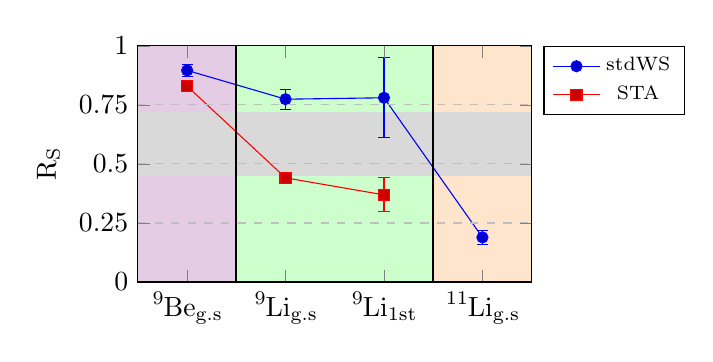
\begin{tikzpicture}
            \begin{axis}[
                width=5cm,
                height=3cm,
                scale only axis,
                ylabel={$\text{R}_{\text{S}}$},
                % minor y tick num=1,
                xticklabels={$\iso{9}{Be}_{\text{g.s}}$, $\iso{9}{Li}_{\text{g.s}}$, $\iso{9}{Li}_{\text{1st}}$, $\iso{11}{Li}_{\text{g.s}}$},
                xtick={0,1,2,3},
                xmin=-0.5, xmax=3.5,
                ymin=0, ymax=1,
                ymajorgrids=true, yminorgrids=false,
                ytick distance=0.25,
                legend style={
                        fill=none,
                        font=\scriptsize,
                        legend pos=outer north east
                    },
                grid style={dashed},
                axis on top,
                ]
                \addplot[fill=black!15, draw=none, forget plot] coordinates {(\pgfkeysvalueof{/pgfplots/xmin}, 0.45) (\pgfkeysvalueof{/pgfplots/xmax}, 0.45)  (\pgfkeysvalueof{/pgfplots/xmax}, 0.72) (\pgfkeysvalueof{/pgfplots/xmin}, 0.72)};
                \addplot+ [
                    error bars/.cd,
                    y dir=both,y explicit,
                ] coordinates {
                        (0, 0.896) +- (0, 0.025)
                        (1, 0.774) +- (0, 0.042)
                        (2, 0.78) +- (0, 0.17)
                        (3, 0.189) +- (0, 0. 031)
                    };
                \addplot+ [
                    error bars/.cd,
                    y dir=both,y explicit,
                ] coordinates {
                        (0, 0.829) +- (0, 0.023)
                        (1, 0.441) +- (0, 0.024)
                        (2, 0.369) +- (0, 0.072)
                    };
                %% Left of axis
                \path[name path=laxis] (\pgfkeysvalueof{/pgfplots/xmin}, 0) -- ( \pgfkeysvalueof{/pgfplots/xmin}, \pgfkeysvalueof{/pgfplots/ymax});
                %% Right of axis
                \path[name path=raxis] (\pgfkeysvalueof{/pgfplots/xmax}, 0) -- ( \pgfkeysvalueof{/pgfplots/xmax}, \pgfkeysvalueof{/pgfplots/ymax});
                %% Left separation
                \addplot[black, thick, name path=right] coordinates {(2.5, \pgfkeysvalueof{/pgfplots/ymin} ) (2.5, \pgfkeysvalueof{/pgfplots/ymax})};
                %% Right separation
                \addplot[black, thick, name path=left] coordinates {(0.5, \pgfkeysvalueof{/pgfplots/ymin} ) (0.5, \pgfkeysvalueof{/pgfplots/ymax})};
                %% Fillings
                % 1 Left
                \addplot[violet!20] fill between [of=laxis and left];
                % 2 Middle
                \addplot[green!20] fill between [of=left and right];
                % 3 Right
                \addplot[orange!20] fill between [of=right and raxis];
                \legend{stdWS, STA}
            \end{axis}
        \end{tikzpicture}
    \end{figure}
    \begin{columns}[c]
        \begin{column}{0.33\linewidth}
            \mycolorbox[1]{box1}{
                What happens with 9Be?
            }
        \end{column}%
        \begin{column}{0.33\linewidth}
            \mycolorbox[1]{box4}{$\text{R}_{\text{S}} $ compatible with litterature
            }
        \end{column}%
        \begin{column}{0.33\linewidth}
            \mycolorbox[1]{box2}{
                $\sim \qty{20}{\percent}$ reduction
                \textbf{GMF} playing a role\\
                Need \textbf{STA}
            }
        \end{column}
    \end{columns}
    }
\end{frame}

\begin{frame}[c]{Conclusions}
    \mycolorbox{box1}{
        Angular distributions for \iso{10,12}{Be}(d,\iso{3}{He}) have been extracted and compared with DWBA
    }
    \vspace{1em}

    \mycolorbox{box2}{
        Found strong sensitivity to nuclear overlap: stdWS or newer STA
    }
    \vspace{1em}

    \mycolorbox{box3}{
        \rs for {\scriptsize $\overlap{\iso{10}{Be}}{\iso{9}{Li}}$} in agreement with systematics
    }
    \vspace{1em}

    \mycolorbox{box4}{
        \rs for {\scriptsize $\overlap{\iso{12}{Be}}{\iso{11}{Li}}$} displays a strong reduction linked to GMF
    }%
\end{frame}

\begin{frame}[t]{Current issues}
    \only<+>{
        \raisebox{0.15em}{\enumitem{1}} Found a quite low efficiency for the ZDD. This lowers the general efficiency since it is mandatory to gate on the heavy particle to identify on the ToF plot.
        \begin{figure}
            \centering
            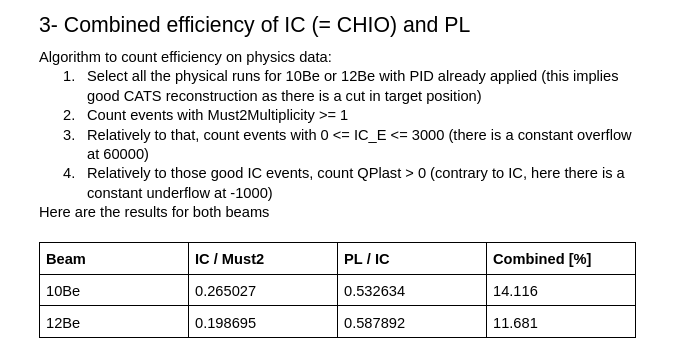
\includegraphics[width=0.8\linewidth]{figures/efficiencies_zdd.png}
        \end{figure}
    }
    \only<+>{
        \raisebox{0.15em}{\enumitem{2}} Experimental and simulated $\sigma$ do not match $\rightarrow$ Work in progress to infer target thickness from this feature.
        \begin{figure}
            \centering
            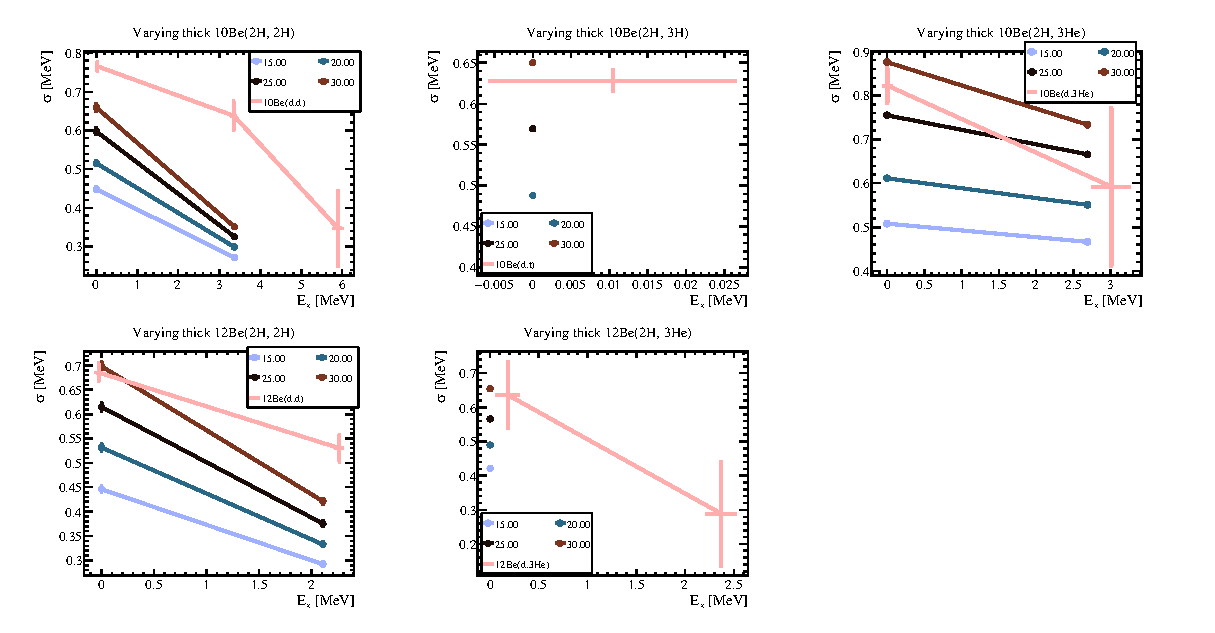
\includegraphics[width=\linewidth]{figures/varying_thick.eps}
        \end{figure}
        Clearly all (but 10Be(d,d)...) agree when thickness $\sim$ \qty{28}{\micro\m}
    }
    \only<+>
    {
        \raisebox{0.15em}{\enumitem{3}} There is an issue with the CsI matching.
        \begin{figure}
            \centering
            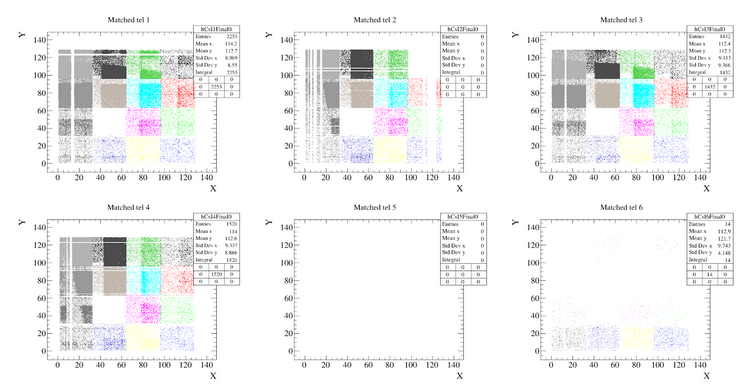
\includegraphics[width=\linewidth]{figures/csi_issue.png}
        \end{figure}
        Check \href{https://docs.google.com/document/d/1u50WcsU5tG_wI53jzvZR6gHnytutCLcSirDCOf8n4us/edit?tab=t.0\#bookmark=id.xomv39b75fdc}{this link} for further info
    }
    \only<+>
    {
        \raisebox{0.15em}{\enumitem{4}} What happens with the B(E2) deformations of \iso{10-12}{Be}?
        \begin{columns}[c]
            \begin{column}{0.5\linewidth}
                \begin{tikzpicture}
                    \node[anchor=south] (image) at (0,0) {
                        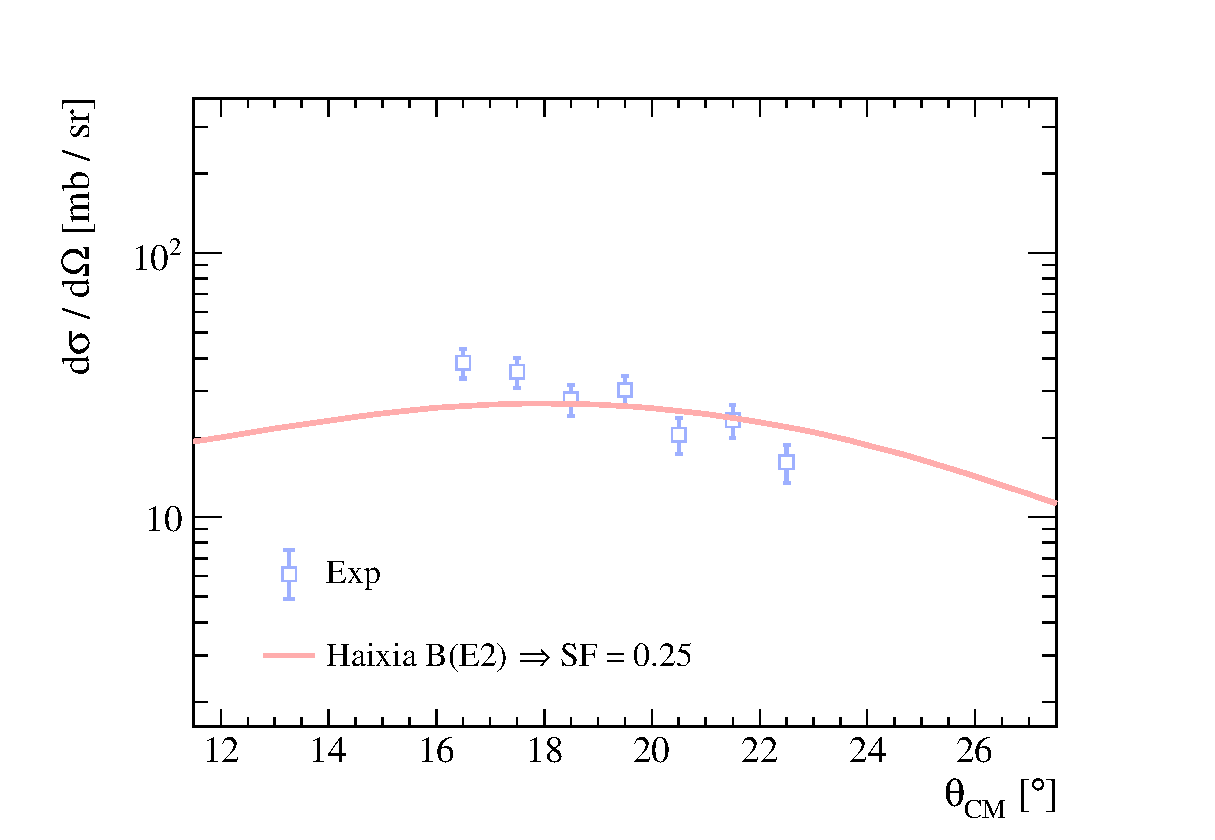
\includegraphics[width=\linewidth]{figures/10Be_dd_g1.eps}
                    };
                    \node at (image.north) {\iso{10}{Be}(d,d)};
                \end{tikzpicture}
            \end{column}\hfill
            \begin{column}{0.5\linewidth}
                \begin{tikzpicture}
                    \node[anchor=south] (image) at (0,0) {
                        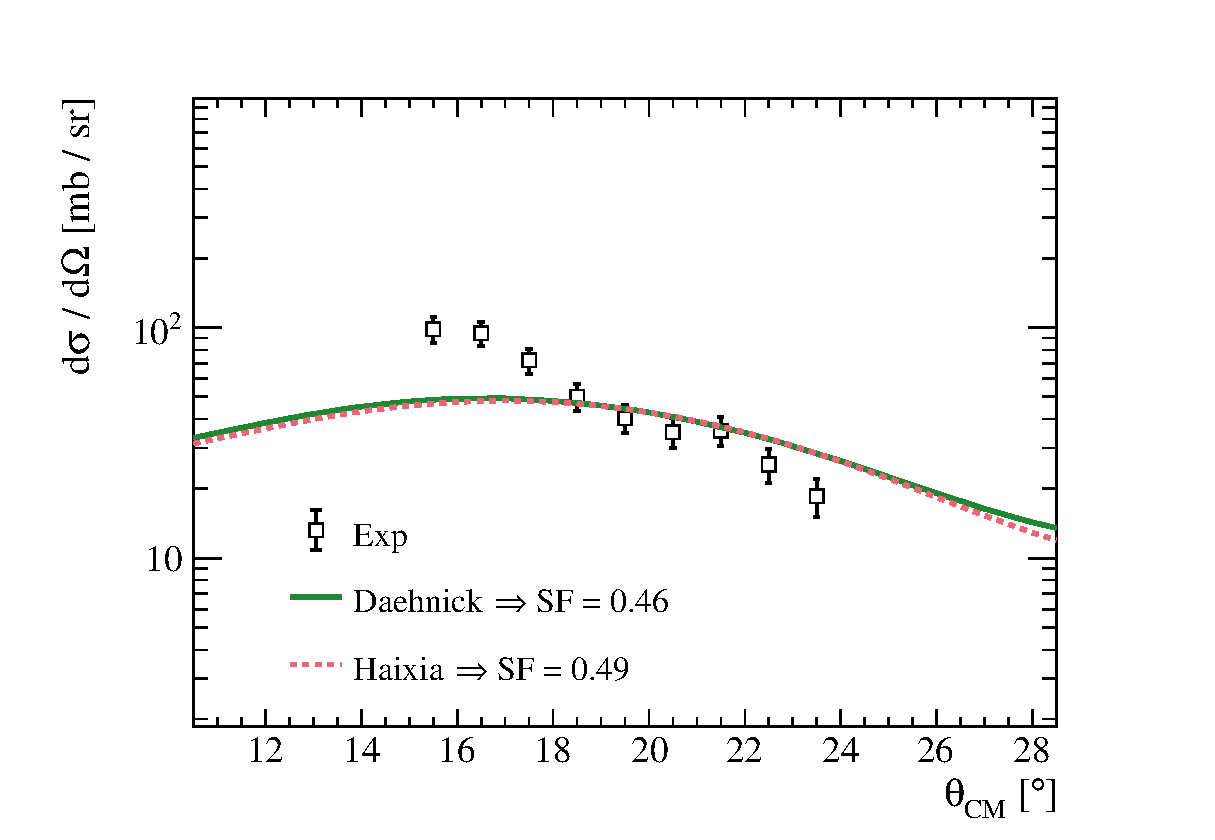
\includegraphics[width=\linewidth]{figures/12Be_dd_g1.eps}
                    };
                    \node at (image.north) {\iso{12}{Be}(d,d)};
                \end{tikzpicture}
            \end{column}
        \end{columns}
        \begin{columns}
            \begin{column}{0.5\linewidth}
                \mycolorbox{box3}{
                    \textbf{Coulomb} deformation:
                    $p_2 = \sqrt{B(E2)}$
                }
            \end{column}
            \begin{column}{0.5\linewidth}
                \mycolorbox{box4}{
                    \textbf{Nuclear} deformation:
                    $p_2 = \beta_2 \cdot R_0$
                    with $R_0 = \qty{1.3}{\femto\m}\cdot A^{1/3}$
                }
            \end{column}
        \end{columns}
    }
\end{frame}

\begin{frame}[plain]{Acknowledgments}
    \begin{columns}[T]
        \begin{column}{0.33\linewidth}
            The E748 collaboration:
            \begin{itemize}\scriptsize
                \item Santiago:\\
                      B. Fernández
                \item LPC-Caen:\\
                      A. Matta\\
                      F. Delaunay\\
                      N. L. Achouri\\
                      F. Flavigny\\
                      J. Gibelin\\
                      M. Marques\\
                      N. Orr
                \item IJCLab:\\
                      D. Beaumel\\
                      M. Assié\\
                      Y. Blumenfeld\\
                      S. Franchoo\\
                      A. Georgiadou\\
                      V. Girard-Alcindor\\
                      F. Hammache\\
                      N. de Séreville\\
                      A. Meyer\\
                      I. Stefan
            \end{itemize}
        \end{column}
        \begin{column}{0.33\linewidth}
            \begin{itemize}\scriptsize
                \item GANIL:\\
                      B. Jacquot\\
                      O. Kamalou\\
                      A. Lemasson\\
                      M. Rejmund\\
                      T. Roger\\
                      O. Sorlin\\
                      J.C. Thomas\\
                      M. Vandebrouck\\
                      B. Bastin\\
                      F. de Oliveira\\
                      C. Stodel
                \item RIKEN:\\
                      S. Koyama\\
                      D. Suzuki
                \item Surrey:\\
                      N. Timofeyuk
            \end{itemize}

        \end{column}
        \begin{column}{0.33\linewidth}
            
\includegraphics[width=0.6\linewidth]{logos/usc_blue.png}\vspace{1em}
            
\includegraphics[width=0.6\linewidth]{logos/lpc.png}\vspace{1em}
            
\includegraphics[width=0.6\linewidth]{logos/ganil.png}\vspace{1em}
            
\includegraphics[width=0.6\linewidth]{logos/ijclab.png}\vspace{1em}
            
\includegraphics[width=0.6\linewidth]{logos/riken.png}\vspace{1em}
            
\includegraphics[width=0.6\linewidth]{logos/surrey.png}\vspace{1em}
        \end{column}
    \end{columns}
\end{frame}

\begin{frame}[noframenumbering, plain]
    \begin{tikzpicture}[remember picture, overlay]
        \node at (current page.center) {
            \usebeamerfont{frame title}
            \textcolor{mainBlue}{Backup}
        };
    \end{tikzpicture}
\end{frame}

\begin{frame}[c,noframenumbering]{Additional: \texorpdfstring{\iso{10}{Be}(p,p)}{10Be(p,p)}}
    This ground state is employed to obtain the number of protons in the target
    \begin{columns}[c]
        \begin{column}{0.5\linewidth}
            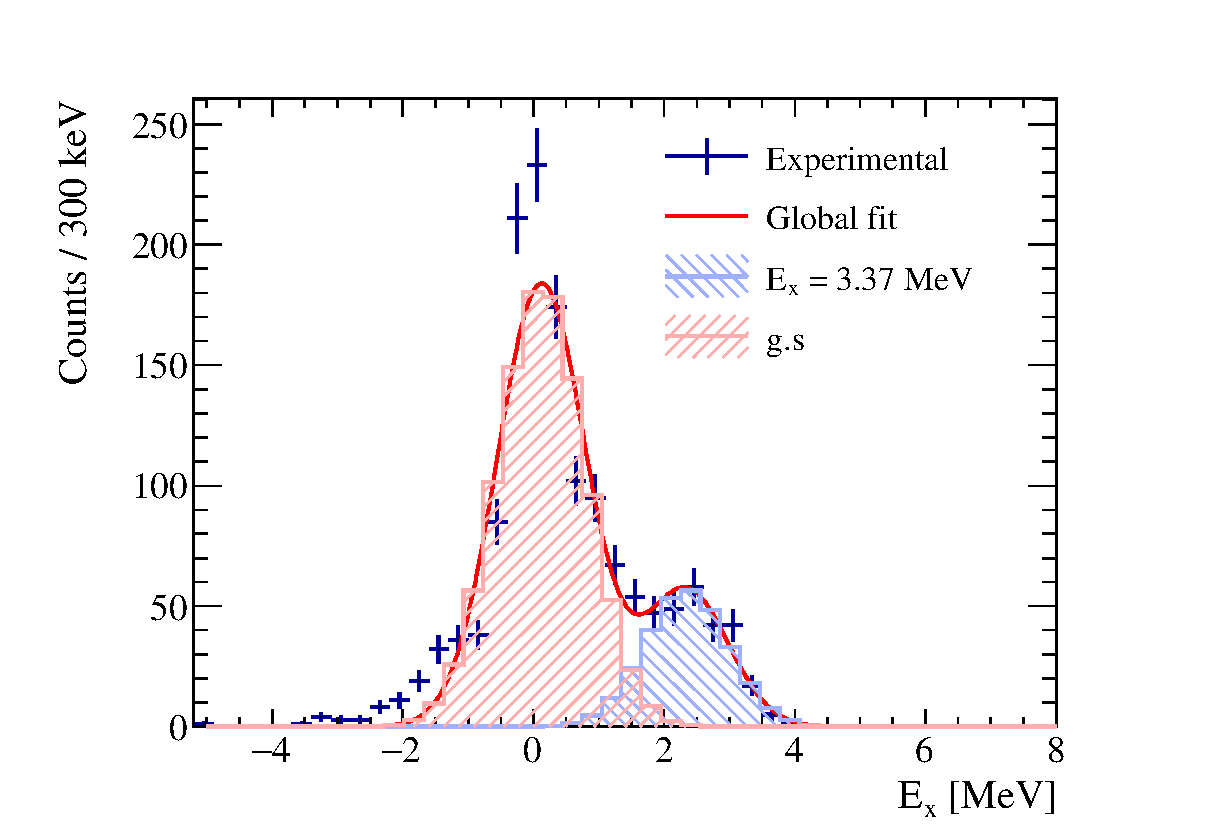
\includegraphics[width=\linewidth]{figures/10Be_pp_fit.eps}
        \end{column}\hfill
        \begin{column}{0.5\linewidth}
            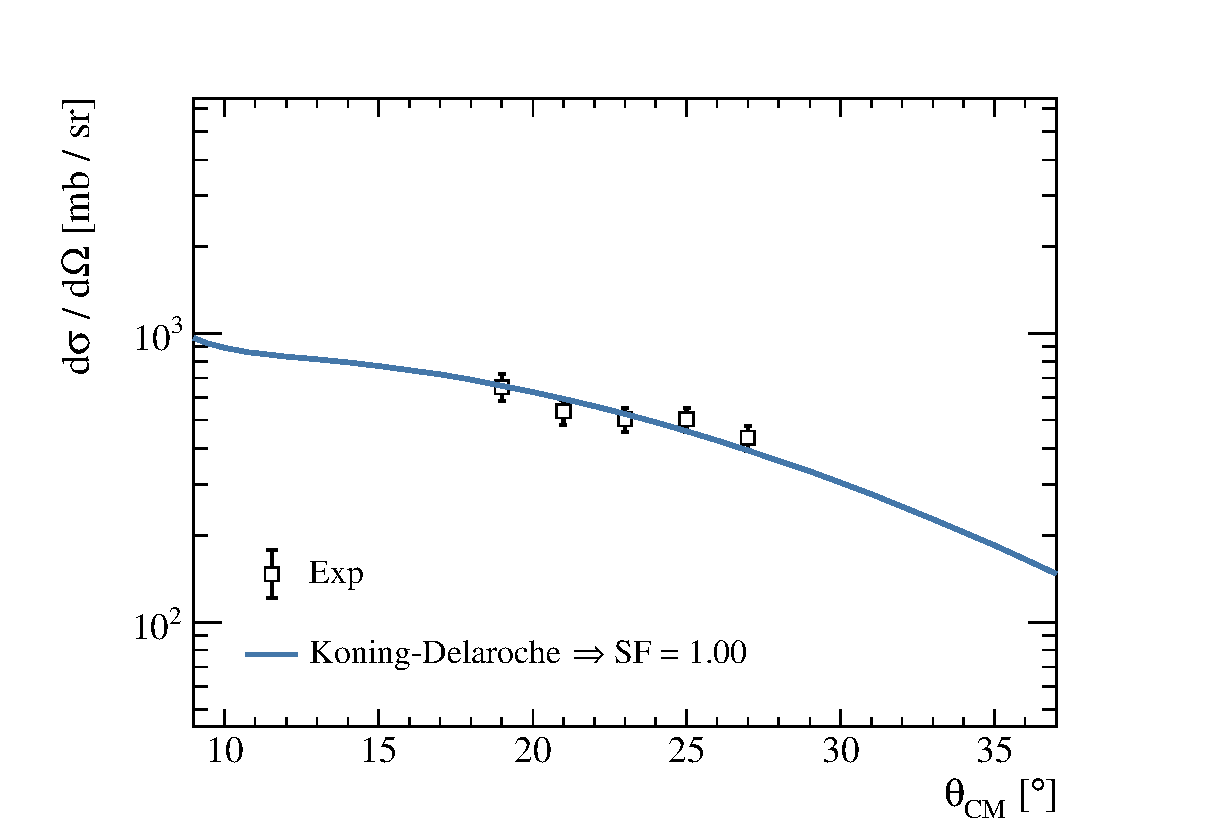
\includegraphics[width=\linewidth]{figures/10Be_pp_g0.eps}
        \end{column}
    \end{columns}

\end{frame}

\begin{frame}[c,noframenumbering]{Additional: \texorpdfstring{\iso{12}{Be}(p,p)}{10Be(p,p)}}
    Same as before but for \iso{12}{Be}
    \begin{columns}[c]
        \begin{column}{0.5\linewidth}
            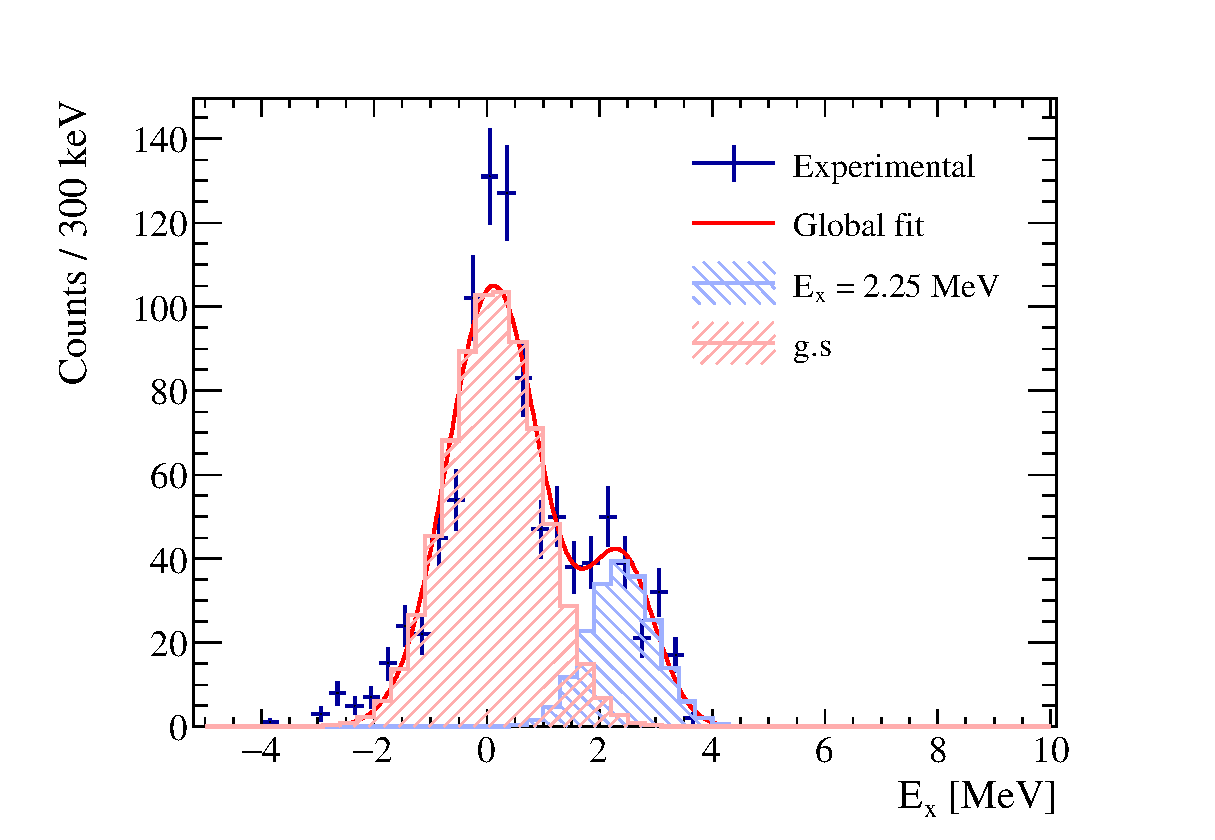
\includegraphics[width=\linewidth]{figures/12Be_pp_fit.eps}
        \end{column}\hfill
        \begin{column}{0.5\linewidth}
            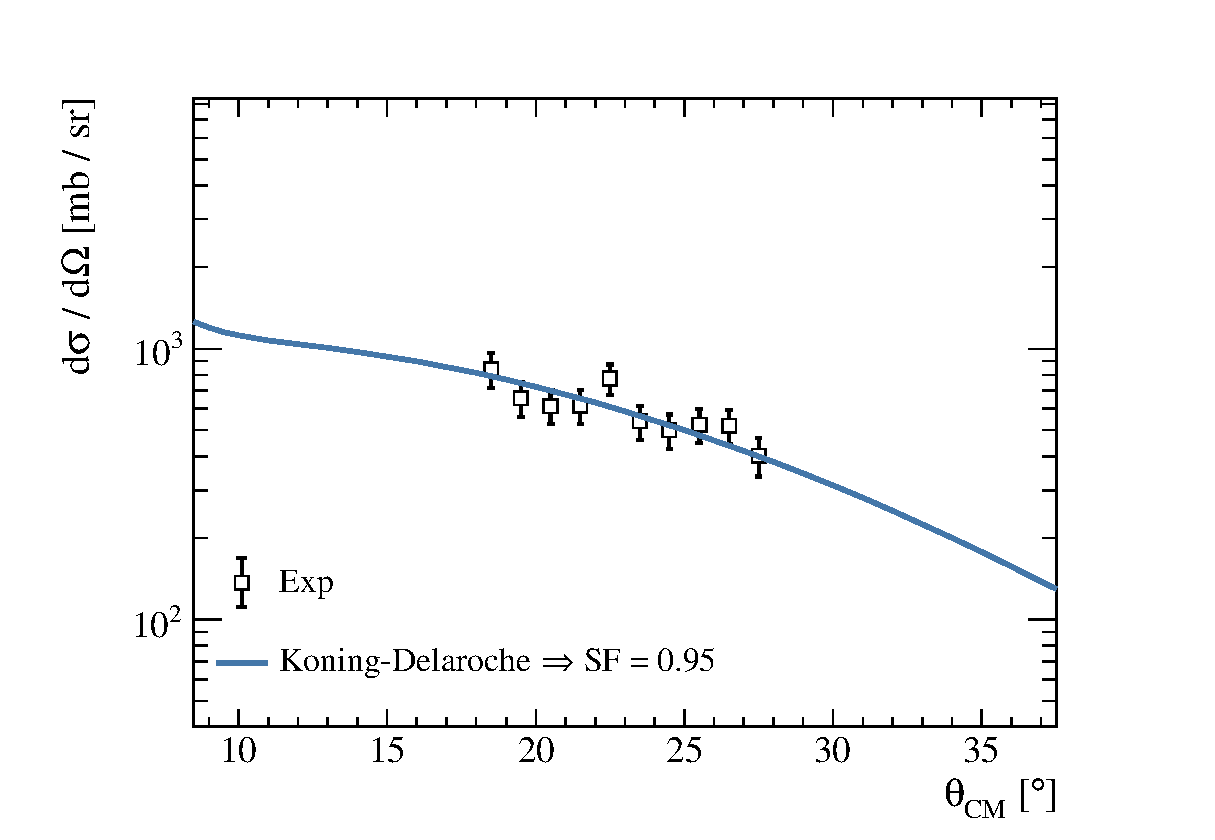
\includegraphics[width=\linewidth]{figures/12Be_pp_g0.eps}
        \end{column}
    \end{columns}

\end{frame}

\begin{frame}[c,noframenumbering]{Additional: inelastic B(E2) with protons}
    The deformations included in the potential are exactly the same as for (d,d) channel.

    \begin{columns}[c]
        \begin{column}{0.5\linewidth}
            \begin{tikzpicture}
                \node[anchor=south] (image) at (0,0) {
                    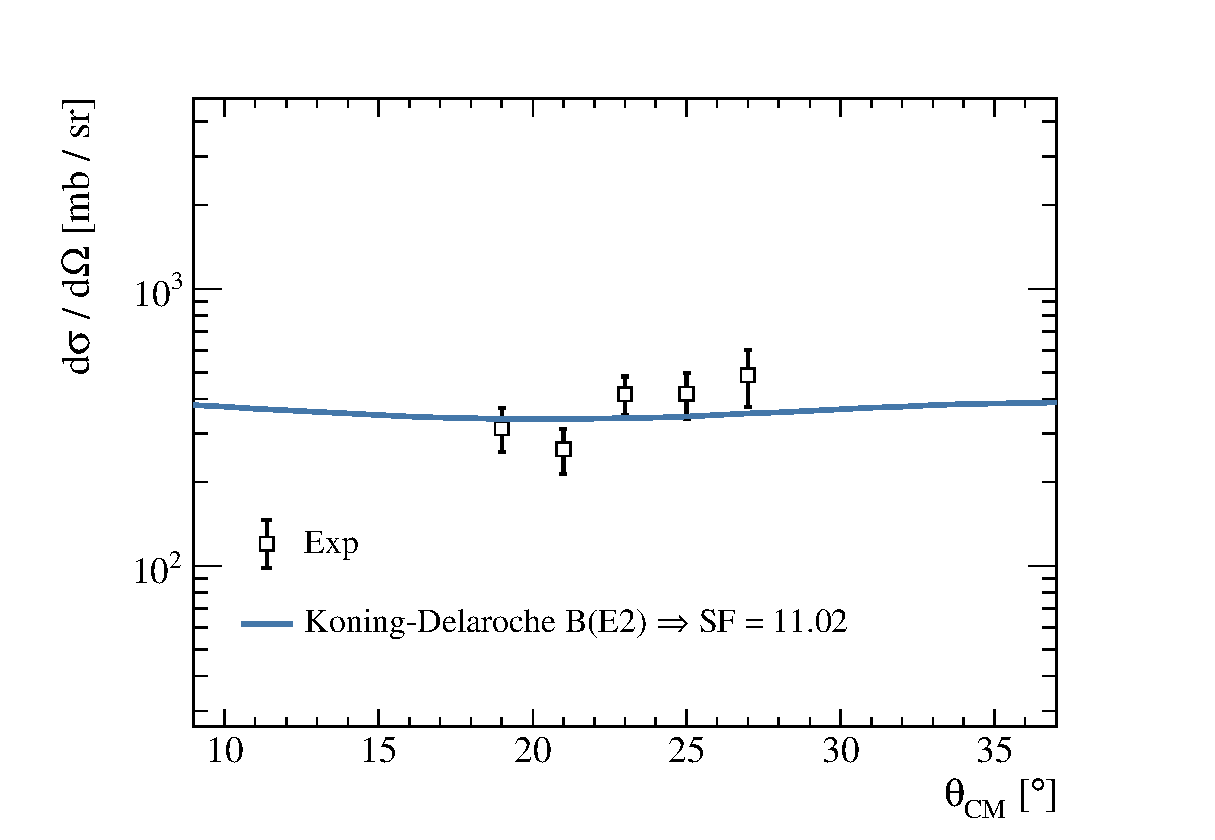
\includegraphics[width=\linewidth]{figures/10Be_pp_g1.eps}
                };
                \node at (image.north) {\iso{10}{Be}(p,p)};
            \end{tikzpicture}
        \end{column}\hfill
        \begin{column}{0.5\linewidth}
            \begin{tikzpicture}
                \node[anchor=south] (image) at (0,0) {
                    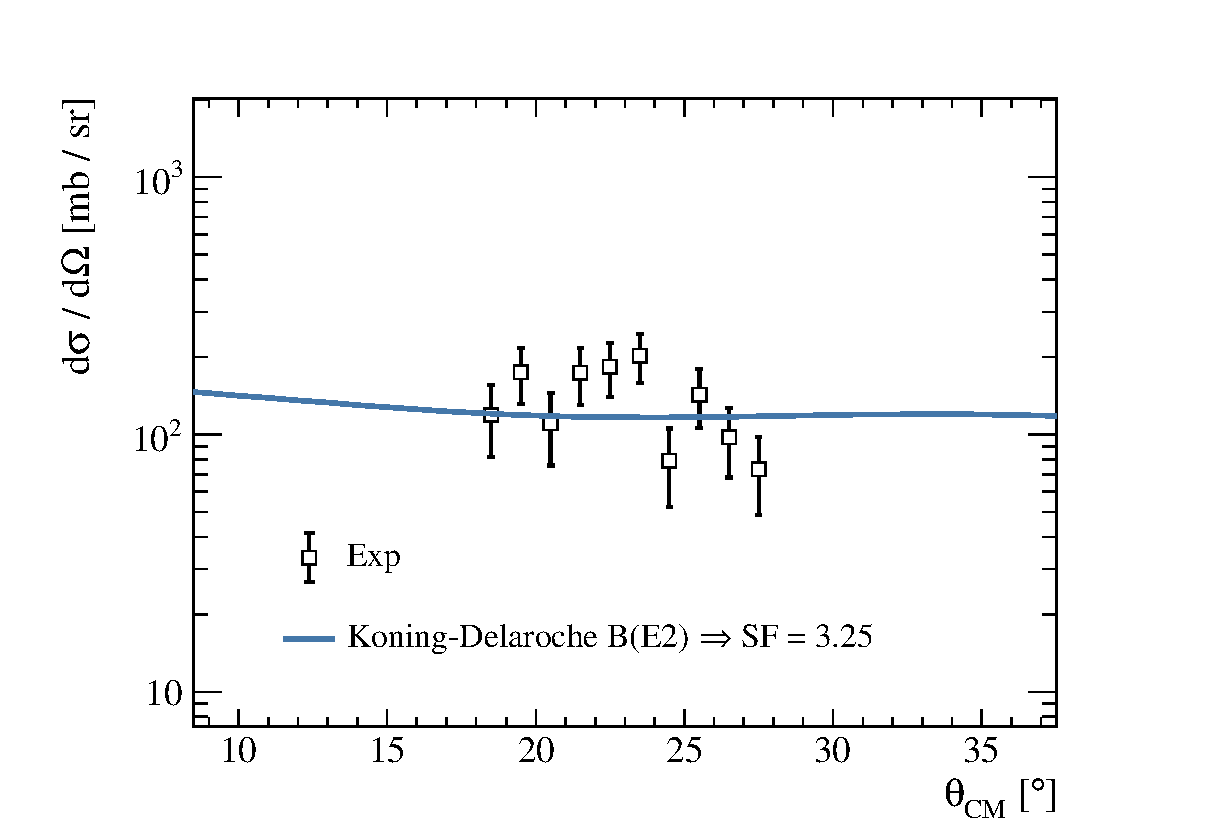
\includegraphics[width=\linewidth]{figures/12Be_pp_g1.eps}
                };
                \node at (image.north) {\iso{12}{Be}(p, p)};
            \end{tikzpicture}
        \end{column}
    \end{columns}
    \mycolorbox{box3}{
        For \iso{10}{Be}(p,p) efficiency is critical: events impinge onto the boundary of the telescope
    }
\end{frame}

\begin{frame}[t, noframenumbering]{Status with light isotopes}
    Several experiments allowed for the extraction of $C^{2}S$ with Li-induced (d, \iso{3}{He}) reactions:
    \vspace{-1.75em}
    \begin{columns}[c]
        \column{0.48\linewidth}{
            \begin{tikzpicture}
                \node[anchor=south west, inner sep=0](image) at (0,0){
                    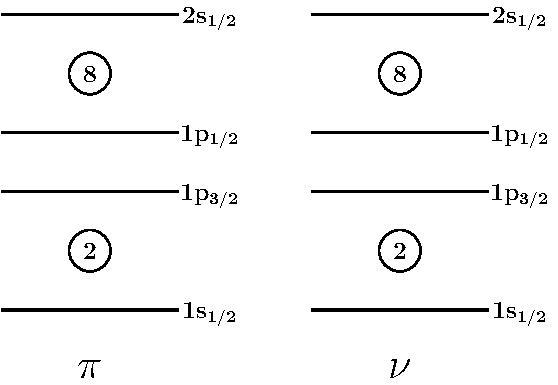
\includegraphics[width=0.75\linewidth]{figures/empty_shell_model.pdf}
                };
                \myscope[false]{
                \node[rectangle, draw, thick, magenta,
                minimum width=1.8cm, minimum height=1.25cm,
                label={[align=center, mainBlue]west:{\small Explored\\ \small region}}] at (0.22, 0.35) {};
                }
            \end{tikzpicture}
        }%
        \column{0.48\linewidth}{
            \begin{figure}
                \begin{tikzpicture}
                    \node[anchor=south west, inner sep=0](image) at (0,0){
                        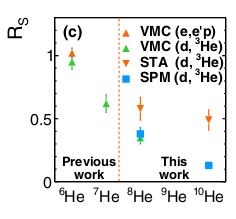
\includegraphics[width=0.75\linewidth]{figures/matta_Rs_Li_He.png}
                    };
                    \myscope[false]{
                    \node[rectangle, draw, very thick, magenta, fit={(0.9, 0.1)(0.8, 0.2)},pin={[mainBlue, pin distance=7mm,
                            pin edge={<-, very thick, black}]75:{\small Unbound!}}
                    ] at (0.9, 0.1) {};
                    }
                \end{tikzpicture}
                \caption{A. Matta \textit{et al.}, Phys. Rev. C 92 (2015)}
            \end{figure}
        }
    \end{columns}
    Several challenges in this region:
    \begin{columns}[T]
        \begin{column}{0.48\linewidth}
            \mycolorbox[0.95]{box3}{
                \enumitem{1} Dealing with \textbf{unbound} nuclei (\iso{10}{He})}
        \end{column}
        \begin{column}{0.48\linewidth}
            \mycolorbox[0.95]{box2}{
                \enumitem{2} Many-body dynamics and/or core excitations}
        \end{column}
    \end{columns}
\end{frame}

\begin{frame}[noframenumbering]{Kinematical lines}
    \begin{columns}[T]
        \begin{column}{0.5\linewidth}
            \begin{tikzpicture}
                \node[anchor=south west, inner sep=0pt] (image) at(0, 0){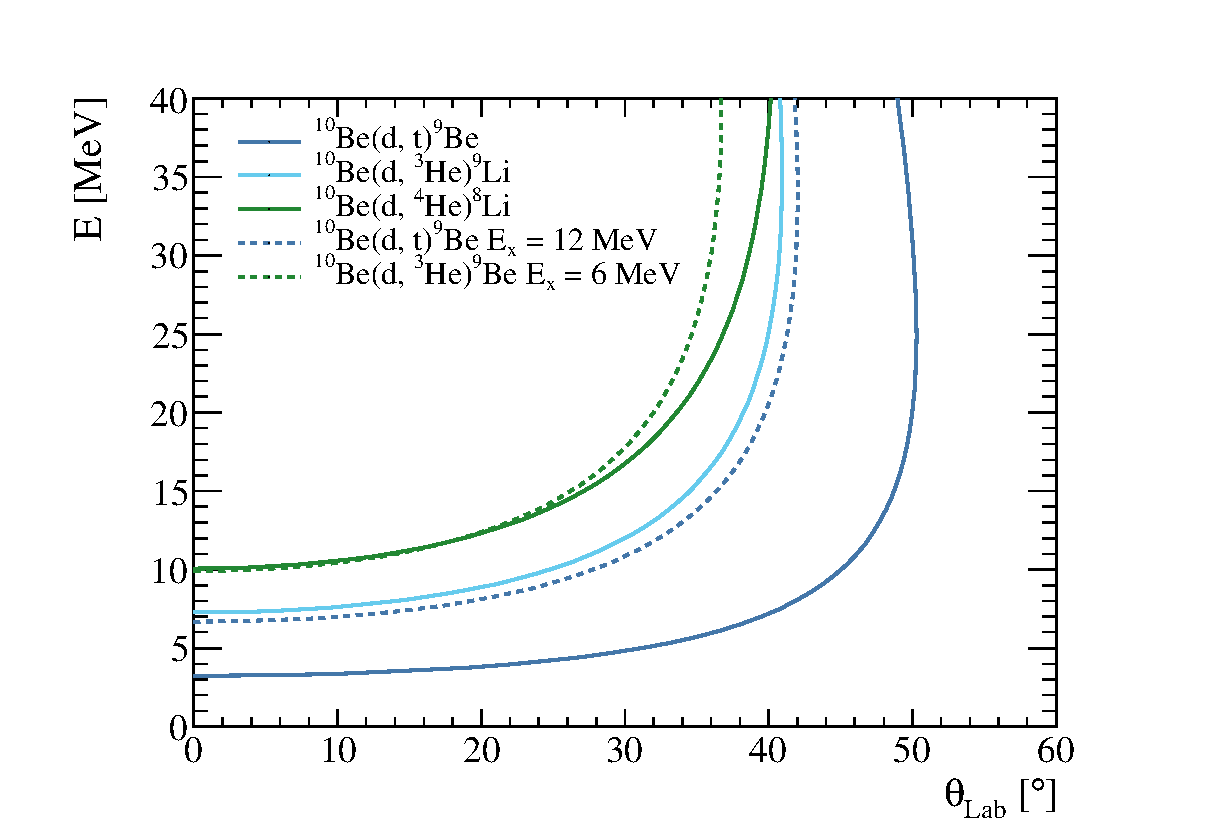
\includegraphics[width=1\linewidth]{figures/kin_10Be.eps}};
                \myscope[false]{
                    \node at (image.north) {\iso{10}{Be}};
                }
            \end{tikzpicture}
        \end{column}
        \begin{column}{0.5\linewidth}
            \begin{tikzpicture}
                \node[anchor=south west, inner sep=0pt] (image) at(0, 0){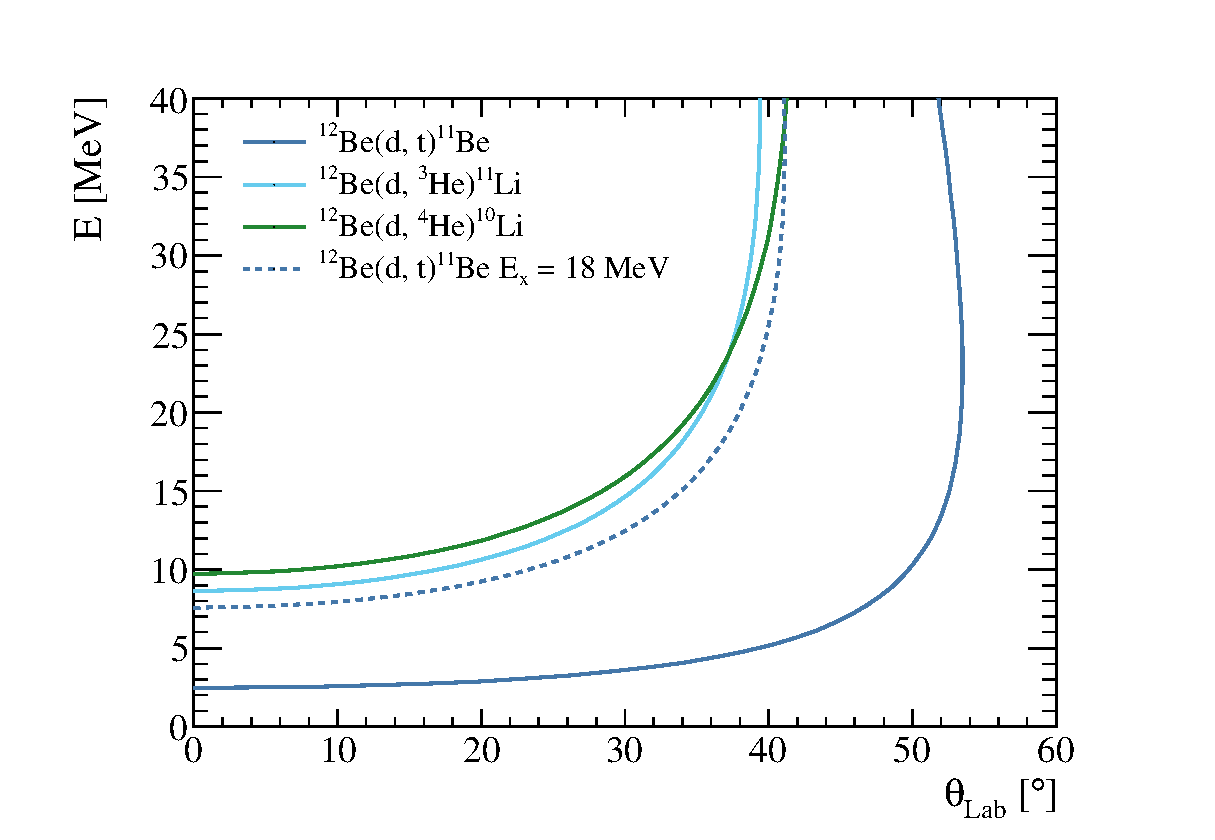
\includegraphics[width=1\linewidth]{figures/kin_12Be.eps}};
                \myscope[false]{
                    \node at (image.north) {\iso{12}{Be}};
                }
            \end{tikzpicture}
        \end{column}
    \end{columns}
\end{frame}

\end{document}